\documentclass[12pt,twoside]{report}
\usepackage{parskip}
\usepackage{comment}
\usepackage{wrapfig}
\usepackage{arev}
\setlength{\parindent}{2em}  % indentation of paragraph

\pagenumbering{arabic}

%%%%%%%%%%%%%%%%%%%%%%%%%%%%%%%%%%%%%%%%%%%%%%%%%%%%%%%%%%%%%%%%%%%%%%%%%%%%%

% Definitions for the title page
% Edit these to provide the correct information
% e.g. \newcommand{\reportauthor}{Timothy Kimber}

\newcommand{\reporttitle}{Automation and Intelligent Optimisation in High Performance Sailing Boats}
\newcommand{\reportauthor}{Doruk Taneli}
\newcommand{\supervisor}{Dr. Pedro Baiz}
\newcommand{\degreetype}{Advanced Computing}

%%%%%%%%%%%%%%%%%%%%%%%%%%%%%%%%%%%%%%%%%%%%%%%%%%%%%%%%%%%%%%%%%%%%%%%%%%%%%

% load some definitions and default packages
%%%%%%%%%%%%%%%%%%%%%%%%%%%%%%%%%%%%%%%%%
% University Assignment Title Page 
% LaTeX Template
% Version 1.0 (27/12/12)
%
% This template has been downloaded from:
% http://www.LaTeXTemplates.com
%
% Original author:
% WikiBooks (http://en.wikibooks.org/wiki/LaTeX/Title_Creation)
%
% License:
% CC BY-NC-SA 3.0 (http://creativecommons.org/licenses/by-nc-sa/3.0/)
% 
%
%%%%%%%%%%%%%%%%%%%%%%%%%%%%%%%%%%%%%%%%%
%----------------------------------------------------------------------------------------
%	PACKAGES AND OTHER DOCUMENT CONFIGURATIONS
%----------------------------------------------------------------------------------------
\usepackage[a4paper,hmargin=2.8cm,vmargin=2.0cm,includeheadfoot]{geometry}
\usepackage{textpos}
\usepackage{natbib} % for bibliography
\usepackage{tabularx,longtable,multirow,subcaption,caption}%hangcaption
\usepackage{fancyhdr} % page layout
\usepackage{url} % URLs
\usepackage[english]{babel}
\usepackage{amsmath}
\usepackage{graphicx}
\usepackage{dsfont}
\usepackage{epstopdf} % automatically replace .eps with .pdf in graphics
\usepackage{backref} % needed for citations
\usepackage{array}
\usepackage{latexsym}
\usepackage[pdftex,pagebackref,hypertexnames=false,colorlinks]{hyperref} % provide links in pdf

\hypersetup{pdftitle={},
  pdfsubject={}, 
  pdfauthor={},
  pdfkeywords={}, 
  pdfstartview=FitH,
  pdfpagemode={UseOutlines},% None, FullScreen, UseOutlines
  bookmarksnumbered=true, bookmarksopen=true, colorlinks,
    citecolor=black,%
    filecolor=black,%
    linkcolor=black,%
    urlcolor=black}

\usepackage[all]{hypcap}


%\usepackage{color}
%\usepackage[tight,ugly]{units}
%\usepackage{float}
%\usepackage{tcolorbox}
%\usepackage[colorinlistoftodos]{todonotes}
% \usepackage{ntheorem}
% \theoremstyle{break}
% \newtheorem{lemma}{Lemma}
% \newtheorem{theorem}{Theorem}
% \newtheorem{remark}{Remark}
% \newtheorem{definition}{Definition}
% \newtheorem{proof}{Proof}


%%% Default fonts
\renewcommand*{\rmdefault}{bch}
\renewcommand*{\ttdefault}{cmtt}



%%% Default settings (page layout)

\setlength{\headheight}{14.5pt}
\pagestyle{fancy}
\renewcommand{\chaptermark}[1]{\markboth{\chaptername\ \thechapter.\ #1}{}} 

\fancyfoot[ER,OL]{\sffamily\textbf{\thepage}}%Page no. in the left on odd pages and on right on even pages
\fancyfoot[OC,EC]{\sffamily }
\renewcommand{\headrulewidth}{0.1pt}
\renewcommand{\footrulewidth}{0.1pt}
\captionsetup{margin=10pt,font=small,labelfont=bf}


%--- chapter heading

\def\@makechapterhead#1{%
  \vspace*{10\p@}%
  {\parindent \z@ \raggedright \sffamily
    \interlinepenalty\@M
    \Huge\bfseries \thechapter \space\space #1\par\nobreak
    \vskip 30\p@
  }}

%---chapter heading for \chapter*  
\def\@makeschapterhead#1{%
  \vspace*{10\p@}%
  {\parindent \z@ \raggedright
    \sffamily
    \interlinepenalty\@M
    \Huge \bfseries  #1\par\nobreak
    \vskip 30\p@
  }}

\allowdisplaybreaks

% load some macros
% Here, you can define your own macros. Some examples are given below.

\newcommand{\R}[0]{\mathds{R}} % real numbers
\newcommand{\Z}[0]{\mathds{Z}} % integers
\newcommand{\N}[0]{\mathds{N}} % natural numbers
\newcommand{\C}[0]{\mathds{C}} % complex numbers
\renewcommand{\vec}[1]{{\boldsymbol{{#1}}}} % vector
\newcommand{\mat}[1]{{\boldsymbol{{#1}}}} % matrix


\date{May 2021}

\begin{document}

% load title page
% Last modification: 2015-08-17 (Marc Deisenroth)
\begin{titlepage}

\newcommand{\HRule}{\rule{\linewidth}{0.5mm}} % Defines a new command for the horizontal lines, change thickness here


%----------------------------------------------------------------------------------------
%	LOGO SECTION
%----------------------------------------------------------------------------------------


\includegraphics[width = 4cm]{./figures/imperial}\\[0.5cm] 

\center % Center remainder of the page

%----------------------------------------------------------------------------------------
%	HEADING SECTIONS
%----------------------------------------------------------------------------------------

\textsc{\Large Imperial College London}\\[0.5cm] 
\textsc{\large Department of Computing}\\[0.5cm] 

%----------------------------------------------------------------------------------------
%	TITLE SECTION
%----------------------------------------------------------------------------------------

\HRule \\[0.4cm]
{ \huge \bfseries \reporttitle}\\ % Title of your document
%Remove in between
\bigskip
{ \Large Background and Progress Report}
%Remove in between
\HRule \\[1.5cm]
 
%----------------------------------------------------------------------------------------
%	AUTHOR SECTION
%----------------------------------------------------------------------------------------

\begin{minipage}{0.4\textwidth}
\begin{flushleft} \large
\emph{Author:}\\
\reportauthor % Your name
\end{flushleft}
\medskip
\begin{flushleft} \large
\emph{CID:}\\
01970609
\end{flushleft}
\end{minipage}
~
\begin{minipage}{0.4\textwidth}
\begin{flushright} \large
\emph{Supervisor:} \\
\supervisor % Supervisor's Name
\end{flushright}
\medskip
\begin{flushright} \large
\emph{Second Supervisor:} \\
Dr. Eric Topham
\end{flushright}
\medskip
\begin{flushright} \large
\emph{Second Marker:} \\
Prof. Julie McCann
\end{flushright}
\end{minipage}\\[4cm]


%----------------------------------------------------------------------------------------
%	FOOTER & DATE SECTION
%----------------------------------------------------------------------------------------
\vfill % Fill the rest of the page with whitespace
Submitted in partial fulfillment of the requirements for the MSc degree in
\degreetype~of Imperial College London\\[0.5cm]

\makeatletter
\@date 
\makeatother


\end{titlepage}



% page numbering etc.
% later: uncomment page numberings
%\pagenumbering{roman}
%\clearpage{\pagestyle{empty}\cleardoublepage}
%\setcounter{page}{1}
\pagestyle{fancy}

\begin{comment}
%%%%%%%%%%%%%%%%%%%%%%%%%%%%%%%%%%%%

\begin{abstract}
Your abstract.
\end{abstract}

%%%%%%%%%%%%%%%%%%%%%%%%%%%%%%%%%%%%
\section*{Acknowledgments}
Comment this out if not needed.

\clearpage{\pagestyle{empty}\cleardoublepage}

\end{comment}

%%%%%%%%%%%%%%%%%%%%%%%%%%%%%%%%%%%%
%--- table of contents
\fancyhead[RE,LO]{\sffamily {Table of Contents}}
\tableofcontents 


\clearpage{\pagestyle{empty}%\cleardoublepage
}
%\pagenumbering{arabic}
%\setcounter{page}{1}
\fancyhead[LE,RO]{\slshape \rightmark}
\fancyhead[LO,RE]{\slshape \leftmark}

%%%%%%%%%%%%%%%%%%%%%%%%%%%%%%%%%%%%

\chapter{Introduction}


Modern sailboats are built by combining bleeding edge science from many areas, including material science for lighter and more durable materials, aero and hydro dynamics for the most efficient designs, and latest sensors for most accurate information. One area that stayed underdeveloped compared to the other parts of the boat is the autopilot. Although autopilot systems have also improved, they are still comparatively crude and low performing.

Shorthanded races are one type of popular competition where there are either one or two crew members, as opposed to full crews that can go up to around ten people. Autopilots are used extensively during these shorthanded races, steering the boat for more than 95\% of the time, while the crew handles other boat work or personal sustenance. Despite carrying out more than 95\% of the steering, autopilots only perform at 80\% of the capability of a professional skipper. Therefore there is a huge potential to gain race winning advantage in shorthanded competitions by improving the autopilots. Jack Trigger \cite{trigger-racing}, who competes in shorthanded races, is providing the data from his boat sensors which makes this project possible. 

The goal of this project is to realize this potential race winning advantage by creating a Machine Learning model, trained by Reinforcement Learning, which will predict the optimal rudder angle using onboard boat sensors. To achieve that, this project will continue the work of former Imperial students and the employees of the partner company, The Data Analysis Bureau (T-DAB) \cite{t-dab}. Extensive work have been done on this project since 2018, mostly focusing on cleaning and preprocessing the available data, plus creating Machine Learning models that predicts the state of the boat and the sea environment.

I, Doruk Taneli, will continue their work, and using the data and code they prepared, I will implement an OpenAI Gym environment in which the Reinforcement Learning will take place. I will then compare the performance of state-of-the-art RL algorithms on this environment, then draw conclusions. If the simulation environment can reproduce the interactions between the rudder, the boat, and the sea realistically enough, the Reinforcement Learning algorithm can potentially learn how to steer a boat better than a human professional.

%\section{Objectives}

%\section{Outcomes}


%%%%%%%%%%%%%%%%%%%%%%%%%%%%%%%%%%%%
\chapter{Background}

\section{State of the Art Autopilots}

The common consumer autopilots work in a very basic way. It either focuses on the boat's heading, using the data from magnetic compass; or focuses on the apparent wind, using the data from the wind sensor usually found at the top of the mast. The autopilot system compares the current reading and the goal reading, and every time the boat diverges from the goal(e.g., by wind or waves), the autopilot compensates by moving the rudder in the opposite way. 

The focus of common consumer autopilots is to keep the boat on the right course. There are also more advanced options, gaining popularity in the last few years, that focus more on performance and racing. These autopilots have some features that imitates how a professional skipper would steer a boat in certain situations. For example: B\&G autopilots \cite{bandg} have gust response feature that quickly recovers from changes in wind, NKE autopilots \cite{nke} have surf mode that promotes the use of waves in downwind angles \cite{yachting_world_2020}, Raymarine autopilots \cite{raymarine} decide on whether to use apparent or true wind depending on wind angle \cite{cruising_world_2019}.

However, these features are all rule based, usually require manual sensitivity tuning, and does not make use of the recent advancement in computing: machine learning. Madintec is the only company that currently uses machine learning in their autopilots for foiling sailboats \cite{madintec}. Foiling sailboats move at extreme speeds, so getting real-time data does not provide enough time for optimal rudder angle calculation. Madintec utilizes a machine learning model to predict the future boat state, and uses that prediction for autopilot decision making \cite{madintec-eric}.

There are no commercially available autopilots that utilize machine learning any further. One notable attempt to use Reinforcement Learning in Sailboat autopilots was done by the RoboSail project \cite{robosail1}. The authors attempted to make a fully autonomous sailing system based on RL, but concluded that it would need several trips around the world for the algorithm to converge \cite{robosail2}. The Robosail team then took on the prevalent approach of rule based autopilots, but let the RL algorithm decide on the parameters and sensitivities instead \cite{robosail3}.

Thanks to the data from Trigger Racing, plus the work of previous students, T-DAB and Imperial College London employees and supervisors, this project aims to tackle the previously unfulfilled challenge of Reinforcement Learning on real-world sailboat autopilots.

\section{Literature Review: RL Algorithms}
In this section, the modern Reinforcement Learning algorithms and the suggested algorithm to be used for our use case in this project is discussed.

\begin{figure}[h]
\centering
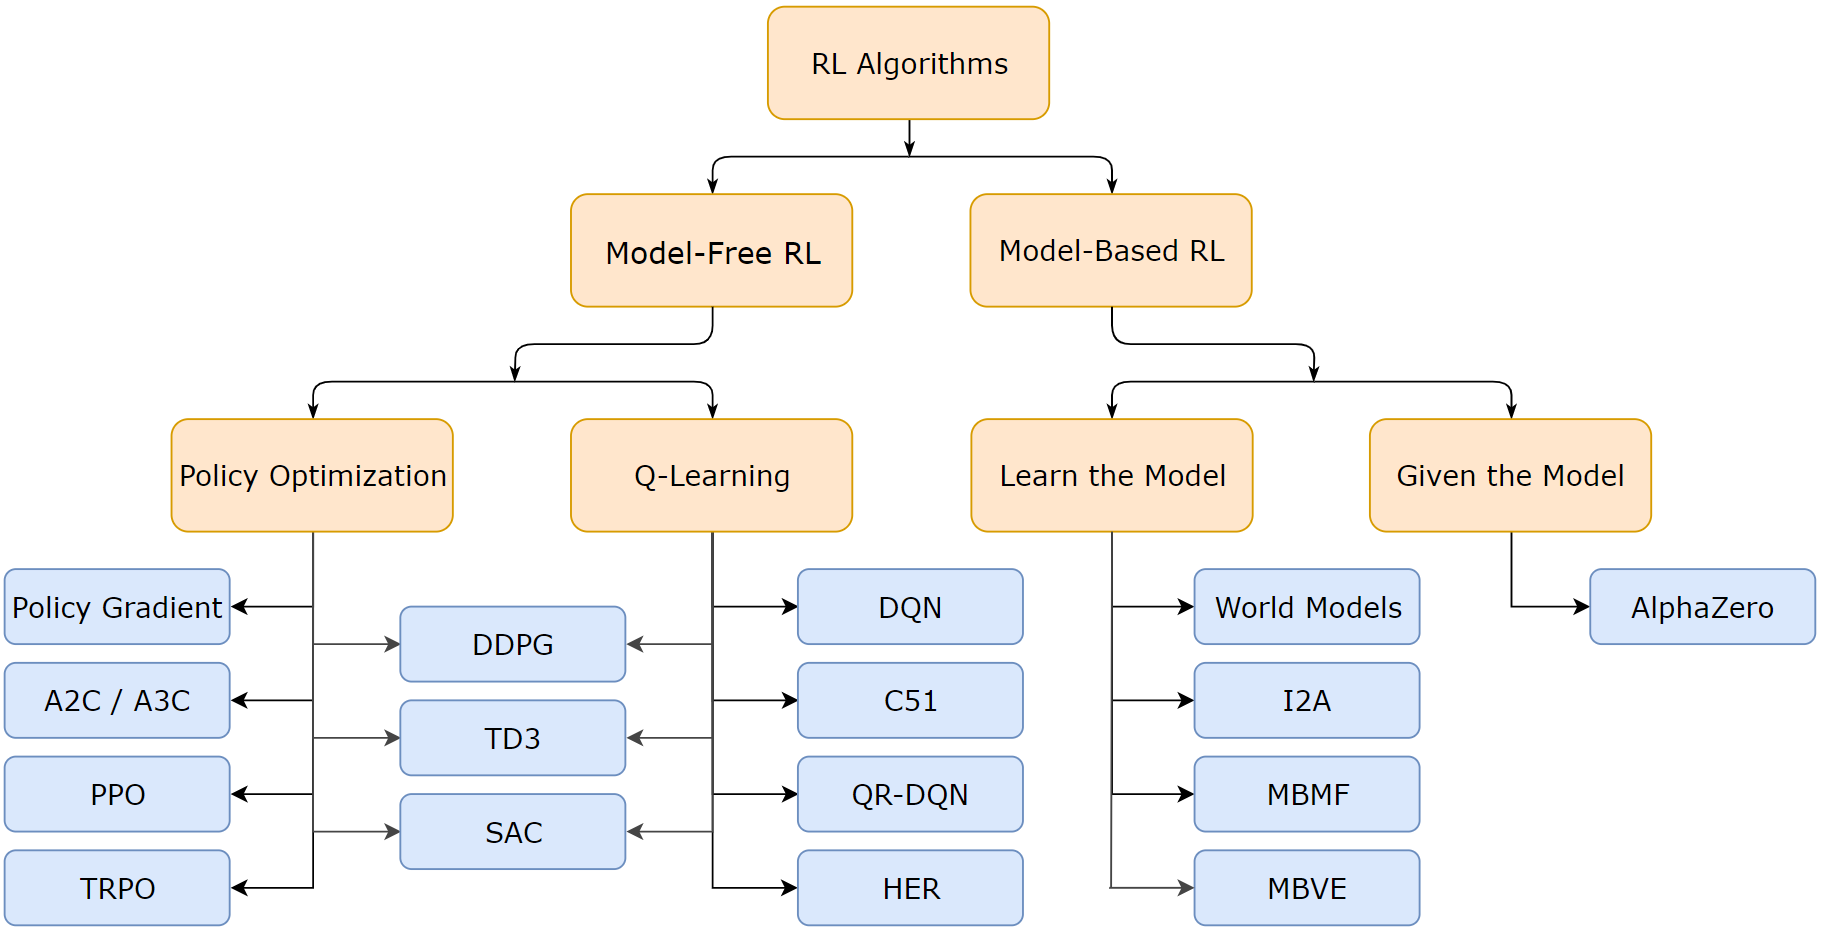
\includegraphics[width = \hsize]{figures/RL algorithms.png}
\caption{A non-exhaustive taxonomy of modern RL algorithms \cite{openai:rl-algs}}
\label{fig:rl-algs}
\end{figure}

An introductory taxonomy of the modern RL algorithms can be seen in Figure ~\ref{fig:rl-algs}. There are two main classes of RL algorithms, Model-Based and Model-Free. In Model-Based algorithms, the algorithms have either access to the environment model, or it learns the environment model. The problem with this branch of algorithms is that usually, the ground truth of the environment is not readily available to the agent. The agent has to learn a simulated environment, then performs poorly on the real environment. This is specifically the case for our project. Furthermore, Model-Based algorithms have not been as extensively developed and tested as the Model-Free algorithms. \cite{openai:rl-algs} Because of these downsides of Model-Based algorithms, I will focus on the Model-Free algorithms for this project.

In Model-Free RL, there are two main techniques: Policy Optimization and Q-Learning. Algorithms such as DDPG, TD3, and SAC - which are state of the are and best suits our use case - uses a hybrid approach of both of these techniques.
DDPG is the first of these algorithms that was developed in 2015, and can be seen as an adaptation of Deep Q-Learning for continuous action spaces. \cite{ddpg} TD3 and SAC were both developed around the same time in 2018. They utilize different tricks to improve DDPG.

\subsection{TD3}
DDPG is prone to overestimating Q-values. Twin Delayed DDPG (TD3) attempts to solve this issue with three tricks: \cite{openai:td3}

\begin{enumerate}
  \item \textbf{Clipped Double-Q Learning:} Instead of one in DDPG, TD3 learns two Q functions, and uses the lesser Q value in the Bellman error loss functions.
  \item \textbf{“Delayed” Policy Updates:} TD3 updates the policy and target networks less frequently than the Q-function. The original paper recommends one policy update for every two Q-function updates.
  \item \textbf{Target Policy Smoothing:} TD3 adds noise to the target action, to make it harder for the policy to exploit Q-function errors by smoothing out Q along changes in action.
\end{enumerate}

In the original TD3 paper, Fujimoto et al. claims that TD3 outperforms the state of the art in every OpenAI gym task tested. \cite{td3} The comparison of the algorithms in different environments can be seen in Figure~\ref{fig:td3-comparisons}.

\begin{figure}[h]
\centering
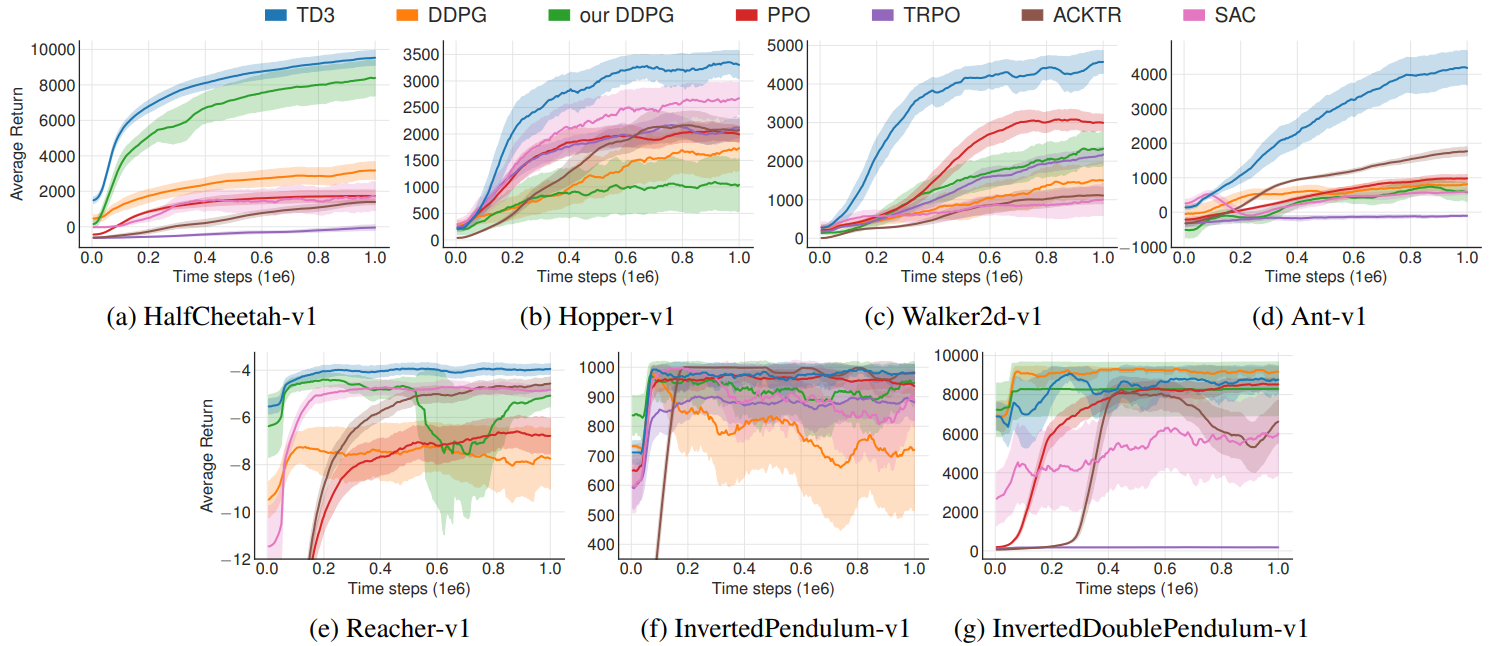
\includegraphics[width = \hsize]{figures/td3 comparison.png}
\caption{Performance comparison of RL algorithms in TD3 paper \cite{td3}}
\label{fig:td3-comparisons}
\end{figure}


\subsection{SAC}
Instead of deterministic policies used in DDPG and TD3, SAC uses stochastic policies. Thus, it is a bridge between stochastic policy optimization and DDPG-style approaches. Like TD3, it uses a few tricks to improve DDPG: \cite{openai:sac}

\begin{enumerate}
  \item \textbf{Entropy Regularization:} The policy is trained to maximize a trade-off between expected return and entropy. This is closely related to exploration-exploitation trade-off: higher entropy results in more exploration, which can accelerate learning and prevent converging to bad local optimum.
  \item \textbf{Next-State Actions:} In SAC, the next-state actions used in the target come from the current policy instead of the target policy.
  \item \textbf{Clipped Double-Q Learning:} Like TD3, SAC makes use of Clipped Double-Q Learning.
  \item \textbf{Target Policy Smoothing:} Although there is no explicit target policy smoothing, since SAC uses a stochastic policy, the noise from the randomness achieves a similar effect.
\end{enumerate}

In the original SAC paper, Haarnoja et al. claims that SAC outperforms the state of the art algorithms in sample-efficiency, asymptotic performance, and stability. \cite{sacOG} The comparison of the algorithms in different environments can be seen in Figure~\ref{fig:sac-comparisons}.

\begin{figure}[h]
\centering
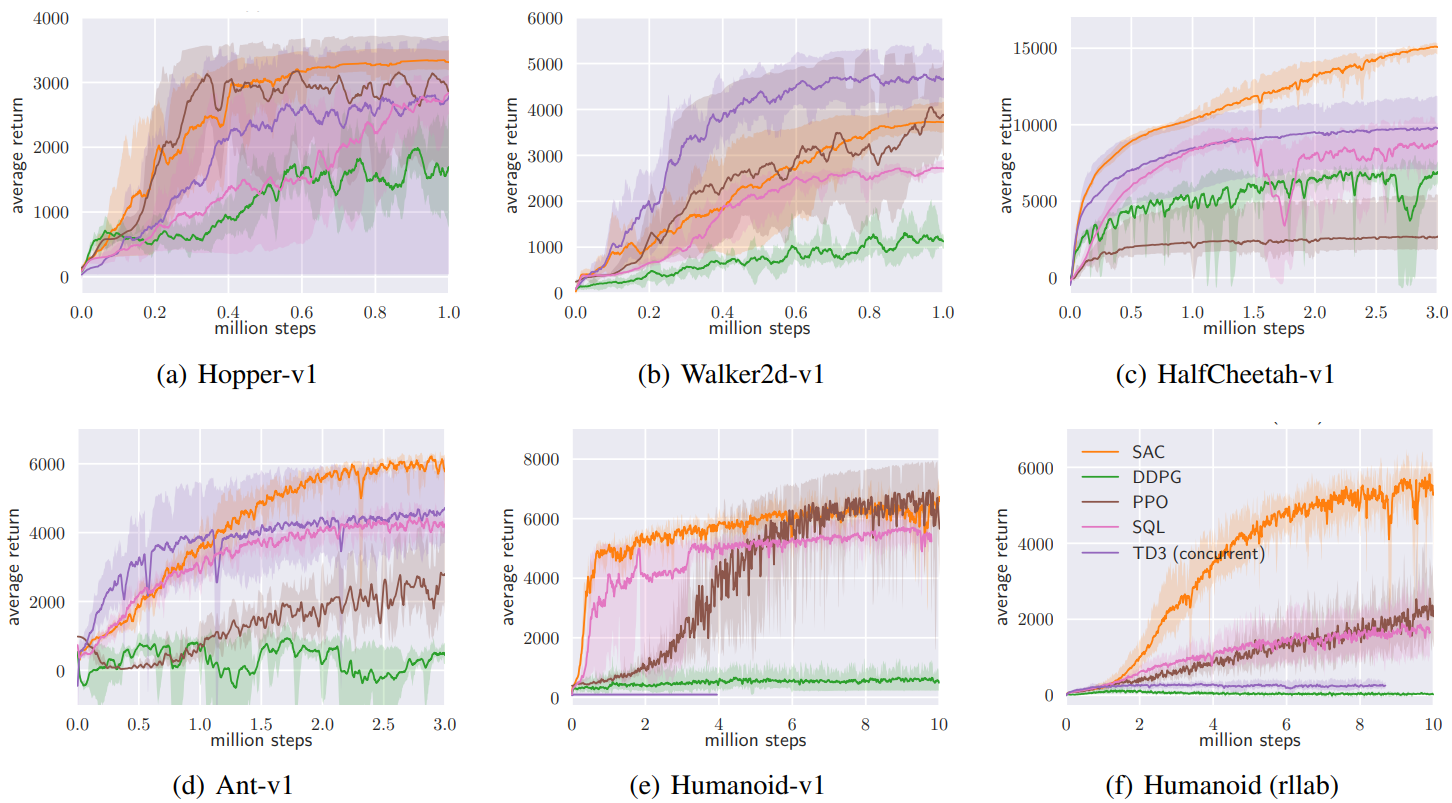
\includegraphics[width = \hsize]{figures/sac comparison og.png}
\caption{Performance comparison of RL algorithms in SAC paper \cite{sacOG}}
\label{fig:sac-comparisons}
\end{figure}

\subsection{Algorithm of Choice}
Interestingly, both SAC and TD3 authors claim that they perform better than each other in their own papers. So a third party benchmark is necessary to be able to compare the two algorithms. A comparison of OpenAI PyTorch implementations of TD3, SAC, and few other algorithms can be seen in Figure \ref{fig:openAI-comparisons}.

\begin{figure}[h]
     \centering
     \begin{subfigure}[b]{0.4\textwidth}
         \centering
         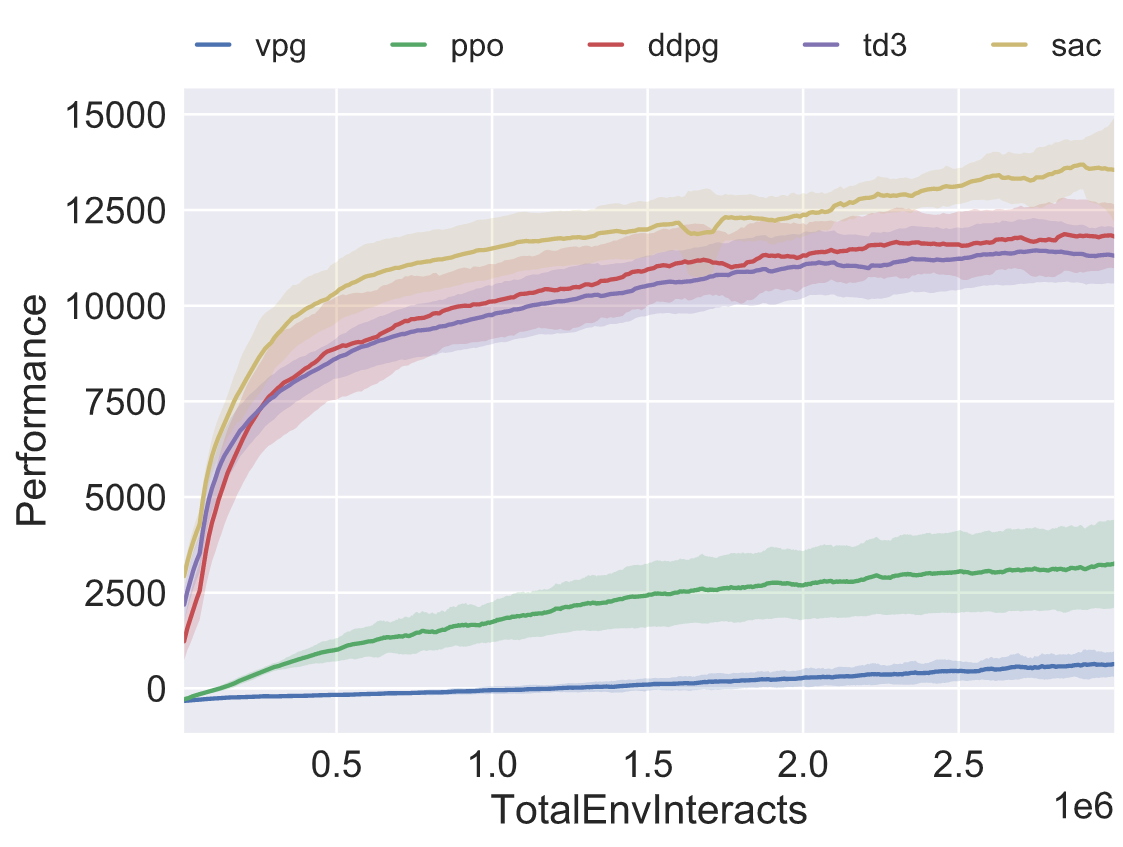
\includegraphics[width=\textwidth]{figures/OpenAI benchmarks/halfcheetah pt.png}
         \caption{HalfCheetah-v3}
     \end{subfigure}
     \quad
     \begin{subfigure}[b]{0.4\textwidth}
         \centering
         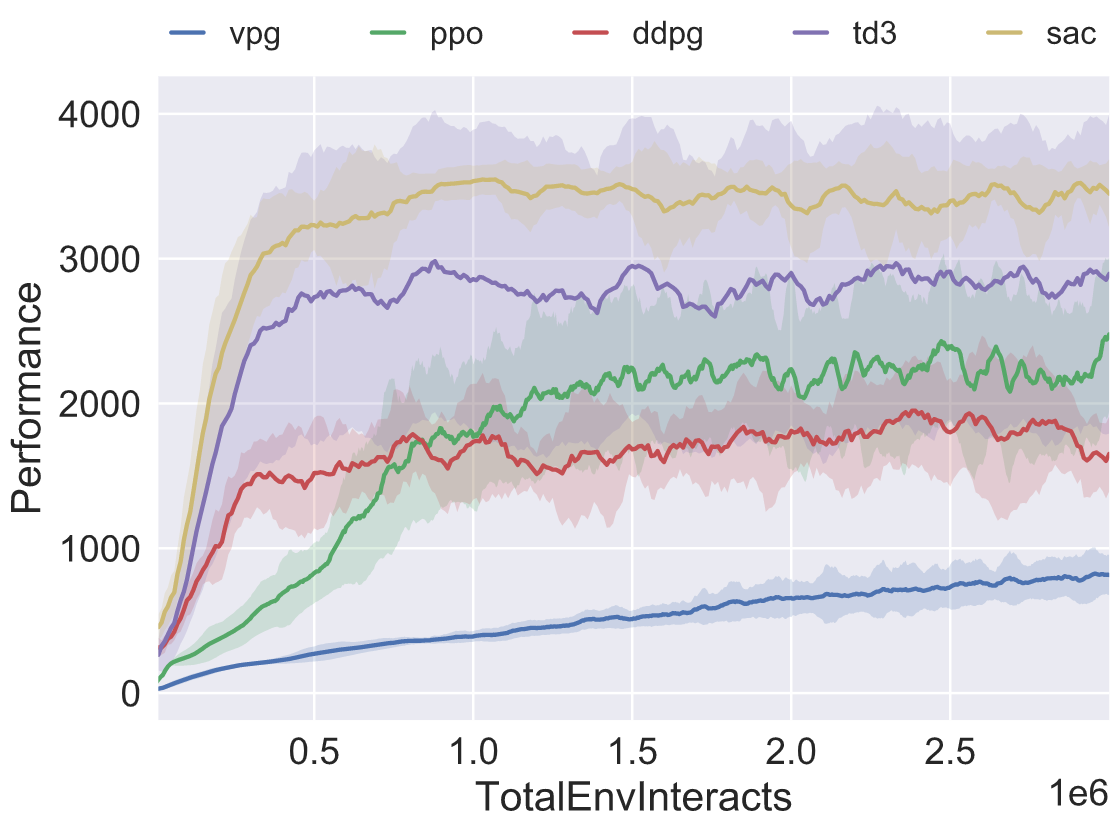
\includegraphics[width=\textwidth]{figures/OpenAI benchmarks/hopper pt.png}
         \caption{Hopper-v3}
     \end{subfigure}
     \quad
     \begin{subfigure}[b]{0.4\textwidth}
         \centering
         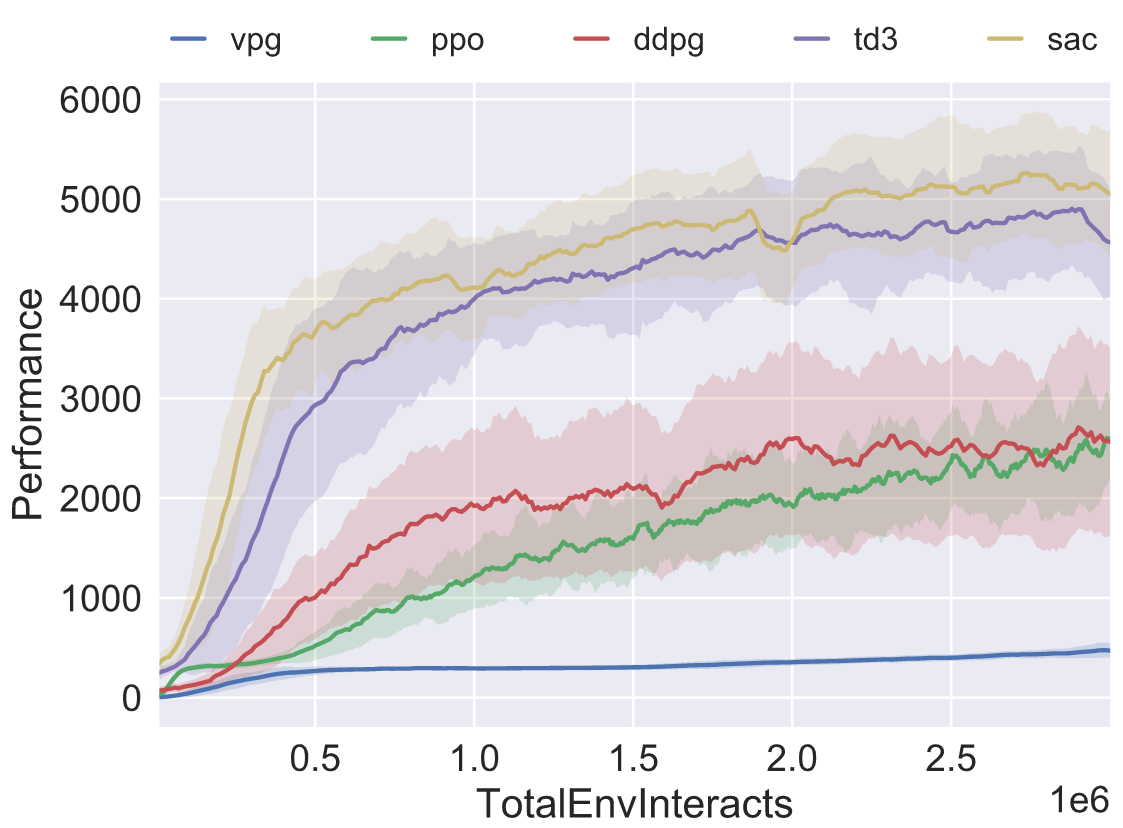
\includegraphics[width=\textwidth]{figures/OpenAI benchmarks/walker pt.png}
         \caption{Walker2d-v3}
     \end{subfigure}
     \quad
     \begin{subfigure}[b]{0.4\textwidth}
         \centering
         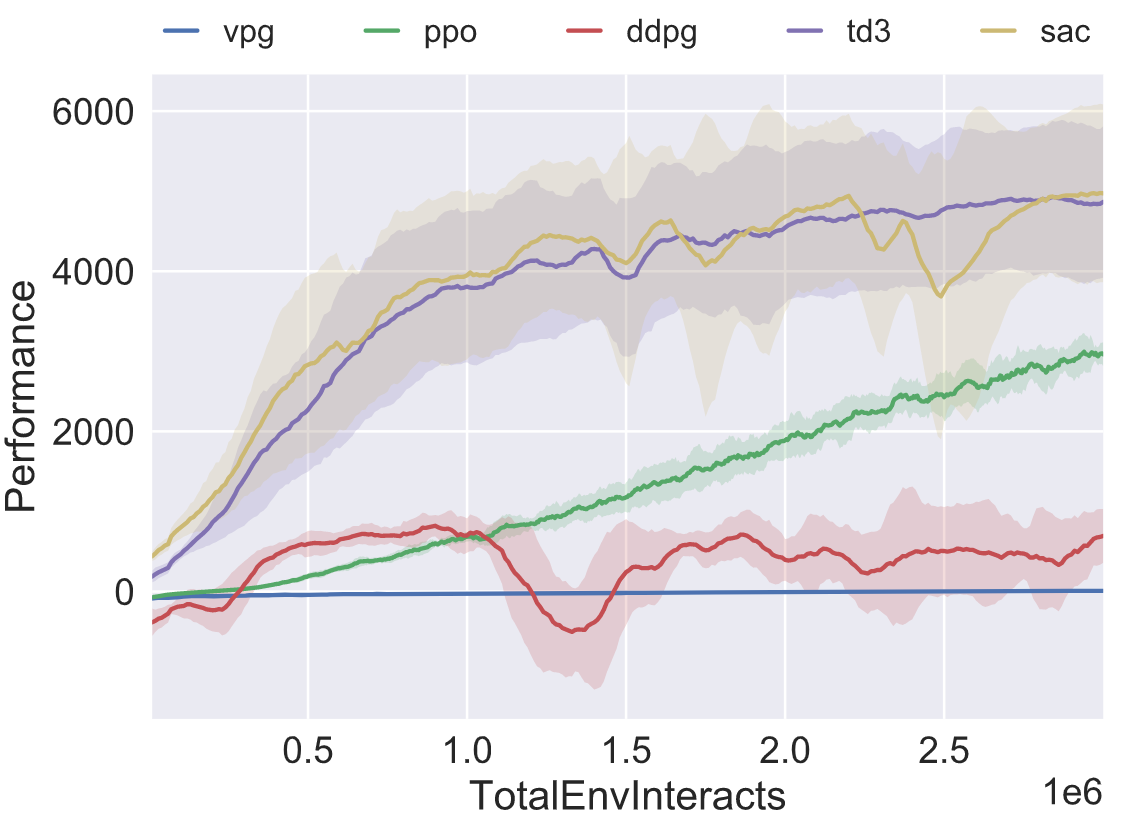
\includegraphics[width=\textwidth]{figures/OpenAI benchmarks/ant pt.png}
         \caption{Ant-v3}
     \end{subfigure}
        \caption{Performance comparison of OpenAI implementations of RL algorithms \cite{openai:bench}}
        \label{fig:openAI-comparisons}
\end{figure}

As can be seen in Figure \ref{fig:openAI-comparisons}, both TD3 and SAC perform very closely to each other, with SAC having a slight advantage over TD3. However one should note that OpenAI implementation of SAC have slight variations that bring it closer to TD3. \cite{openai:sac-code}

The advantage of TD3 is that it performs really close to SAC, with less complexity and less hyperparameters to tune. However, the second iteration of SAC from the original authors automatically tunes the problematic temperature hyperparameter, reducing the problem of hyperparameter tuning, making the algorithm more stable among different seeds and environments, and performs well even in the worst case, which is important for real life use cases. \cite{sacOG}

Because of these reasons, the suggested algorithm to be used for the Reinforcement Learning Approach is Soft Actor-Critic (SAC).

\subsection{Recent Advancement: Truncated Quantile Critics}

Truncated Quantile Critics (TQC) is a novel algorithm whose original paper was published in May 2020 \cite{tqc-paper}. TQC aims to solve the overestimation bias in continuous off-policy learning by combining three ideas: distributional representation of a critic, truncation of critics prediction, and ensembling of multiple critics. The authors claim that TQC outperforms the current state of the art in all the environments they tested. The comparison of the algorithms can be seen in Figure \ref{fig:tqc-comparison}.

\begin{figure}[h]
\centering
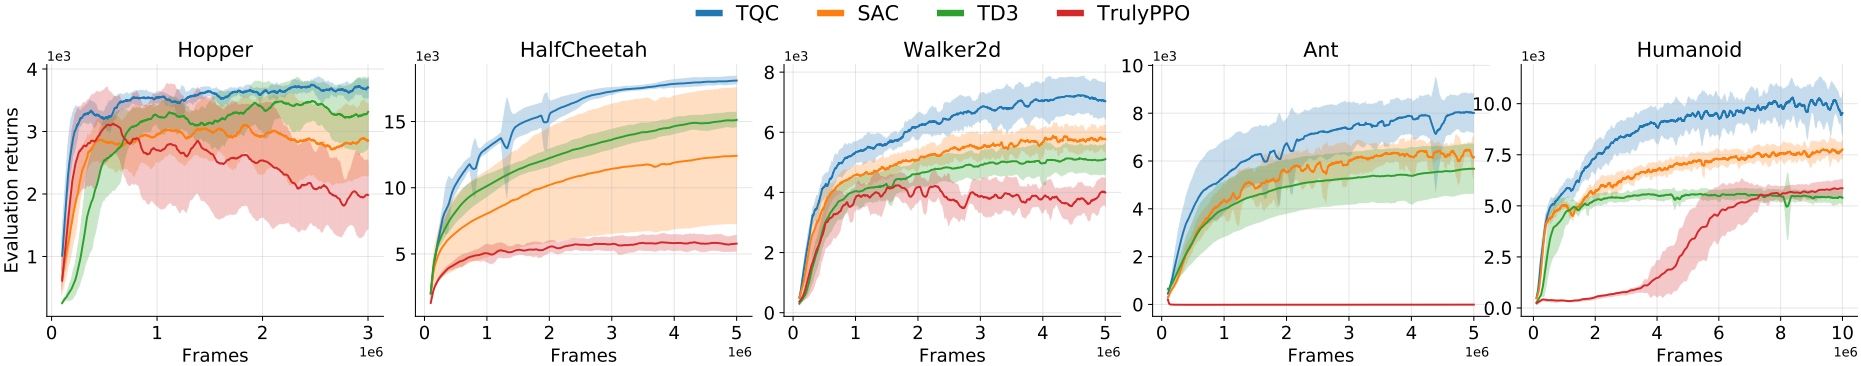
\includegraphics[width = \hsize]{figures/tqc comparison.png}
\caption{Average performance of RL algorithms on MuJoCo Gym Environments \cite{tqc-paper}}
\label{fig:tqc-comparison}
\end{figure}

TQC is not as thoroughly tested as the current state of the art, but it shows promising results, especially in the harder environments. Although it is in beta, there is an implementation of TQC publicly available. Therefore, this new advancement in continuous RL algorithms will definitely be incorporated in this project.

\section{Previous Student Work}
The "Automation and Intelligent Optimisation in High Performance Sailing Boats" project started in 2019. Birk Ulstad and Roman Kastusik started working on the project simultaneously. Birk Ulstad took the Supervised Learning Approach, whereas Roman Kastusik took the Reinforcement Learning Approach to the problem. Following their work, Stanislas Hannabelle continued working on the supervised learning approach in late 2019. In 2020, Charles Metz continued the Reinforcement Learning work of Roman Kastusik. A very brief summary of each students work is presented below.
%I, Doruk Taneli, will be picking up where Birk, Roman, Stanislas, and Charles left off and  further improve the project.

\subsection{Birk Ulstad}
Birk's goal was to develop a supervised machine learning model that predicts the rudder angle set by Jack Trigger on the Concise 8 boat, using the previous data recorded during races by the existing sensors on the boat. \cite{birk}

Birk Ulstad converted the available raw, partially corrupted data to processable csv data. He then cleaned the csv data by removing the irrelevant and corrupted parts, analysing outliers and applying smoothing. Next, he normalized, reframed, and downsampled the data to get it ready for the supervised learning model.

\begin{figure}[h]
\centering
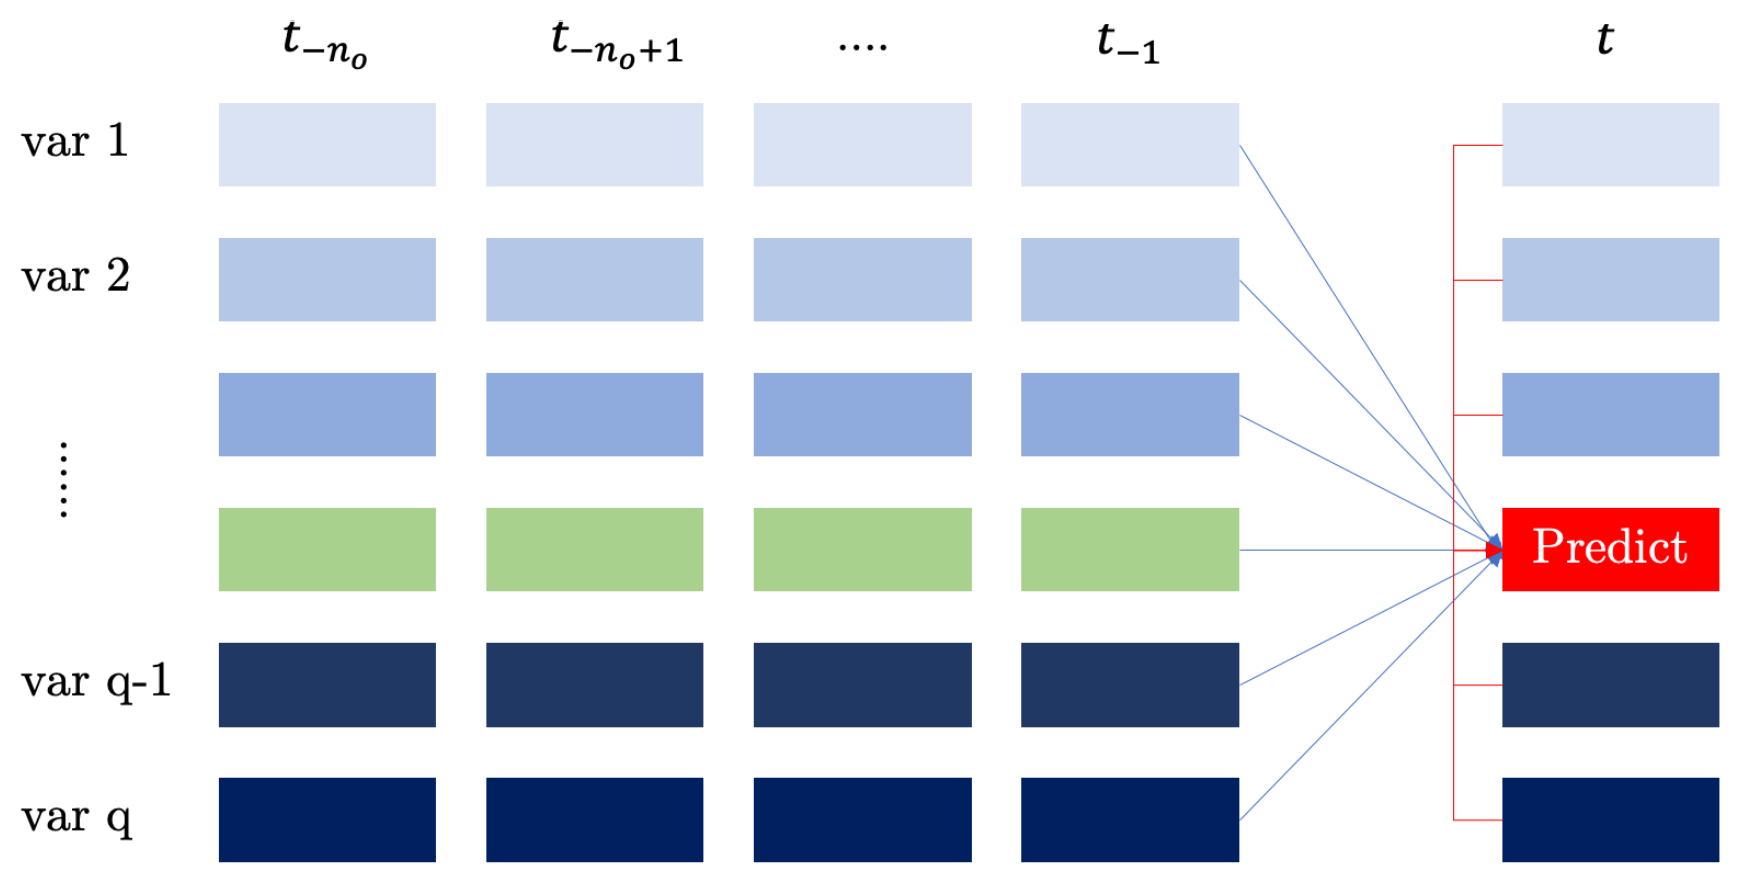
\includegraphics[width = 0.7\hsize]{figures/Birk Ulstad LSTM prediction.png}
\caption{Birk Ulstad's LSTM prediction methods}
\label{fig:birk lstm}
\end{figure}

For the model, Birk preferred a two stateful LSTM layers, each followed by a dropout layer to prevent overfitting. The prediction plan of the model can be seen in Figure~\ref{fig:birk lstm}. The original plan was to use both past values of the feature set until time t-1 (blue arrows) and the current values at time t (red arrows) to predict the rudder angle. However he only managed to get blue arrow predictions to work, and used those while discussing his results.

Birk concluded that his model architecture is able to predict the rudder angle produced by a human within a couple of degrees. His other notable observations were: 
\begin{itemize}
  \item The model is able to predict the autopilot's rudder angle with much less error compared to a human's rudder angle. Birk explained this as "Learning a univariate rule-based function [of an autopilot] is easier than learning the multivariate function that maps human sensory input to human rudder output".
  \item Downsampling the available data to 5 Hz from 25 Hz is a good middle ground between training time and RMSE. 
  \item An input sequence length between 5-15 seconds provides an optimal trade-off between training time and prediction accuracy.
\end{itemize} 

\subsection{Roman Kastusik}
Roman's objective was to utilize reinforcement learning to increase the autopilots' performance, potentially beyond human level. To achieve this, he trained an LSTM state estimator to simulate the boat's behavior using Jack Trigger's race data, and created a reinforcement learning algorithm that would interact with said simulation environment. \cite{roman}

\begin{wrapfigure}{R}{0.55\textwidth}
\centering
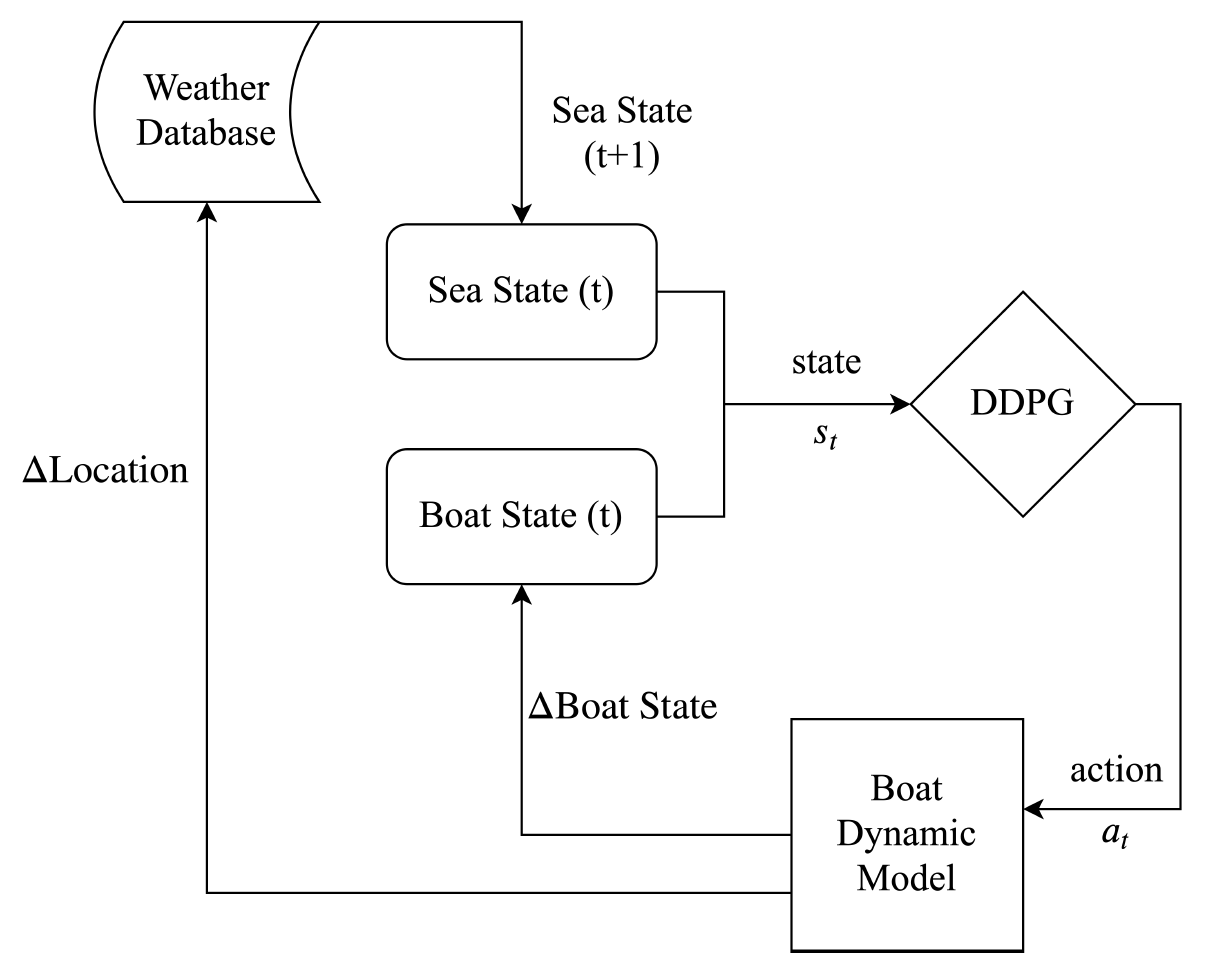
\includegraphics[width = 0.54\textwidth]{figures/roman data flow.png}
\caption{Roman Kastusik's RL data flow}
\label{fig:roman dataflow}
\end{wrapfigure}

Roman started with some data analysis, data cleaning, and scaling on Jack Trigger's race data. He then used  used this data to train the simulation environment that would be used for the reinforcement learning algorithm. The data flow around the simulation environment and the reinforcement learning algorithm can be found in Figure \ref{fig:roman dataflow}.

He also did research about the recent advancements in reinforcement learning, and created an RL algorithm utilizing Deep Deterministic Policy Gradients, Actor-Critic Networks and Experience Replay.

Roman concluded that due to the poor performance of the simulation environment, it was not possible to realize the full potential of the reinforcement learning algorithm. Charles Metz later continues his work and improves the simulation environment.

\subsection{Stanislas Hannabelle}
Stanislas' goal was to improve the results of Birk Ulstad's supervised learning approach to the problem. He further cleaned the dataset using a tack\footnote{Tacking is a sailing maneuver where the boat changes direction by turning its head towards and through the wind so that the direction from which the wind blows changes from one side of the boat to the other, allowing progress in the desired direction. \cite{wiki:tack}} detection system, did hyperparameter and bayesian optimization, and compared GRU and LSTM models. He was able to reduce the Root Mean Squared Error from 3.493 degrees of Birk's final model to 1.096 degrees, and reduced the computational time needed for rudder angle prediction. \cite{stan}

\begin{figure}[h]
\centering
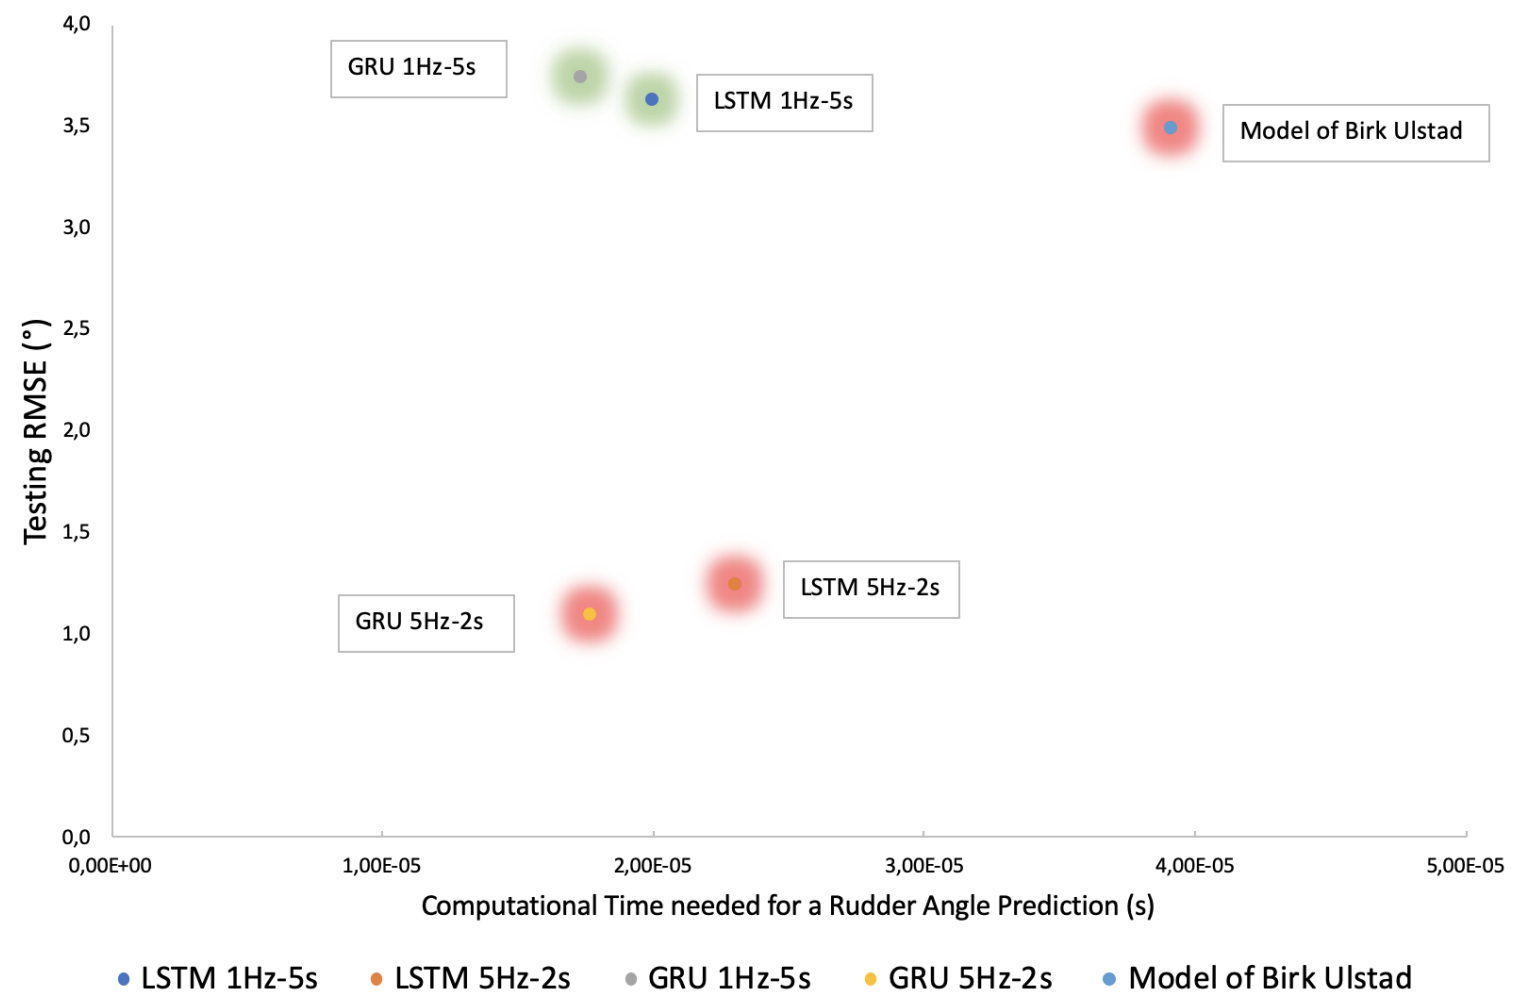
\includegraphics[width = 0.8\hsize]{figures/stan results.png}
\caption{Stanislas Hannabelle's improvements on supervised learning approach}
\label{fig:stan results}
\end{figure}

Stanislas further cleaned the available dataset by training a classifier to remove tacks, and manually removing the abnormal sailing conditions such as extremely light wind. With the new dataset, he performed the grid search shown in Table \ref{tbl:stan grid} for best sampling frequency (Hz) and input sequence length (seconds). He then performed bayesian optimization for LSTM and GRU models for 1Hz-5s and 5hz-2s parameters. After training and testing with the best hyperparameters he found, Stanislas got the results in Figure \ref{fig:stan results}.

\begin{table}[h]
\centering
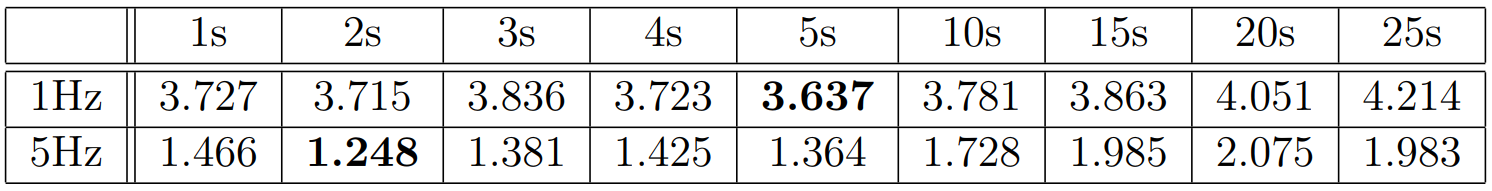
\includegraphics[width=\linewidth]{figures/stan grid search.png}
\caption{validation RMSE for sampling frequency and input length combinations}
\label{tbl:stan grid}
\end{table}

With his best model 'GRU 5Hz-2s', Stanislas reduced the testing RMSE of Birk's model by approximately 68\% while cutting the required training time in half. Stanislas' model was able to predict the rudder angle produced by a human by around 1 degree. His other success was to reduce the computational time needed for rudder angle prediction so that the model can be implemented live in onboard autopilots.

\subsection{Charles Metz}
Charles' goal was to improve the state estimator model Roman suggested, so it can reliably reproduce the behaviour of a sailing boat in its sea environment. His main idea was that instead of using 1 model to predict n sea and boat features like Roman, he used n models to predict n different features, which lead to very significant improvement. \cite{charles}

\begin{wraptable}{R}{0.55\textwidth}
\centering
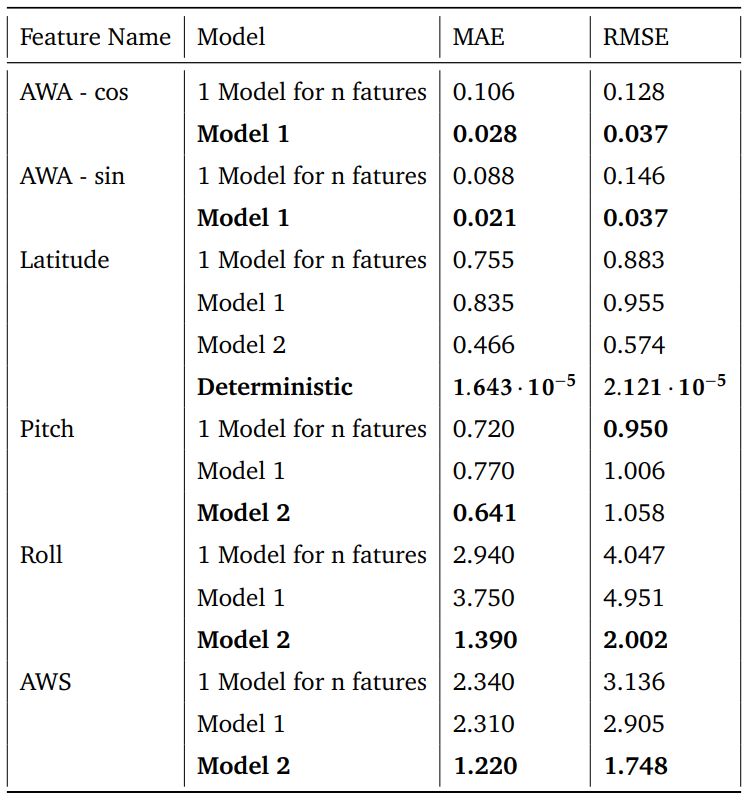
\includegraphics[width=0.54\textwidth]{figures/charles results.png}
\caption{Charles' prediction method results}
\label{tbl:charles results}
\end{wraptable}

Charles had a new dataset available, so he started by applying similar cleaning and preprocessing steps to this new dataset. He noticed that some of the features can be derived mathematically from other features such as true wind, apparent wind, and boat speed. He decided to calculate those features mathematically, then trained n separate models for n remaining features. He tried 2 different models, model 1 has two final dense layers whereas model 2 has only one final dense layer.

He concluded that in general, deterministic mathematical derivations has the least error, followed by model 2, then model 1, and lastly single model for n features. He tested model 2 in only some of the features, but it performed better in every feature tested. Error rate of different prediction methods for some of the boat features can be seen in Table \ref{tbl:charles results}. Charles envisions that after n models for n features are individually optimised, they can be integrated into a reinforcement learning framework.



%%%%%%%%%%%%%%%%%%%%%%%%%%%%%%%%%%%%
\chapter{Progress}
\section{RL Framework}
After the Background Research, the planned framework to use was OpenAI's Spinning Up framework. They provide clean implementations of modern RL algorithms, and a basic interface to apply the algorithms to OpenAI Gym environments, then plot the results. However, OpenAI Spinning Up has some downsides and lack some important features that would be helpful during this project.

\subsection{RL Algorithm Implementation Differences} \label{RLF:imp-diff}
Spinning Up's main focus is education. Therefore the algorithm implementations are stripped down from the proposed versions from the original papers, so the algorithms would be easier to read and understand. Although this is good for education, the resulting algorithms do not perform up to their potential due to their simplicity. The performance of SAC which is the algorithm of choice for this project, used on different Gym environments can be seen in Figure \ref{fig:spinup-SAC}.

\begin{figure}[h]
     \centering
     \begin{subfigure}[t]{0.32\textwidth}
         \centering
         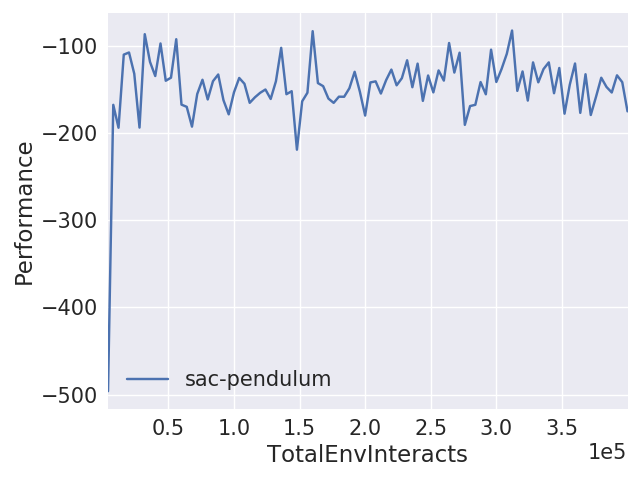
\includegraphics[width=\textwidth]{figures/rl-framework/sac-pendulum.png}
         \caption{Pendulum-v0 (Very Easy)}
     \end{subfigure}
     \hfill
     \begin{subfigure}[t]{0.32\textwidth}
         \centering
         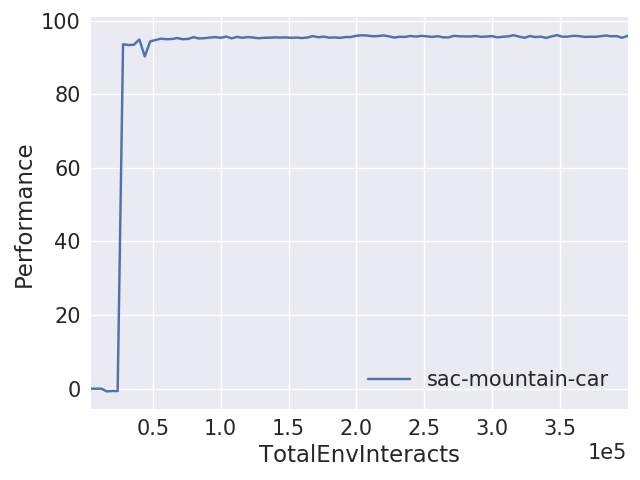
\includegraphics[width=\textwidth]{figures/rl-framework/sac-mountain-car.png}
         \caption{MountainCarContinuous-v0 (Easy)}
     \end{subfigure}
     \hfill
     \begin{subfigure}[t]{0.32\textwidth}
         \centering
         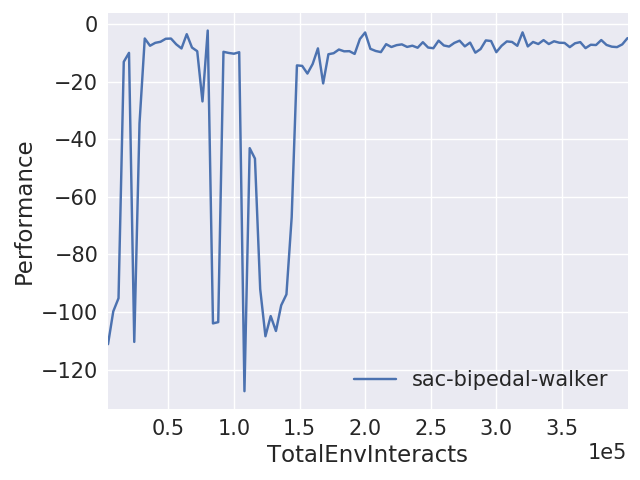
\includegraphics[width=\textwidth]{figures/rl-framework/sac-bipedal-walker.png}
         \caption{BipedalWalker-v3 (Hard)}
     \end{subfigure}
        \caption{Performance of Spinning Up implementation of SAC on different environments, using default parameters}
        \label{fig:spinup-SAC}
\end{figure}

Spinning Up implementation performs well and converges quickly on easy environments, but it provides disappointing results on the harder BipedalWalker-v3 environment. SAC is expected to have better exploration and achieve better results on BipedalWalker-v3 environment before 300.000 environment interacts \cite{gym-leaderboard}. But it never managed to escape a local minimum for a long period of training time. Considering our sailing environment will be pretty complex, Spinning Up implementation of SAC is not suitable for use on this project.

\subsection{RL Framework Features} \label{RLF:framework-features}

Spinning Up Framework lacks some important features for Reinforcement Learning. First, it does not support continuing training of a previously trained agents. This is problematic in a few ways: it costs precious time and resources to train agents from scratch every time, plus even if models are trained again from ground up, no two reinforcement learning runs will be identical because of the noise or stochasticity in the algorithms.

\begin{wrapfigure}{R}{0.5\textwidth}
\centering
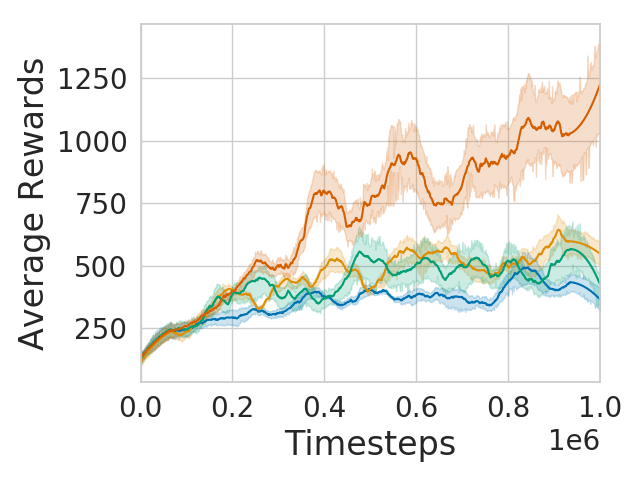
\includegraphics[width = 0.48\textwidth]{figures/rl-framework/hyperparameter-ddpg.png}
\caption{DDPG on Walker2d-v1 with random hyperparameters \cite{hyperparameter-ddpg}}
\label{fig:hyperparameter-ddpg}
\end{wrapfigure}

The second lacking feature is that there is no hyperparameter optimization support. Hyperparameters can cause huge difference in performance \cite{hyperparameter-ddpg}. A comparison of DDPG on Walker2d-v1 with random hyperparameters can be seen in Figure \ref{fig:hyperparameter-ddpg}. The best and worst performing hyperparameters have approximately 3-fold average reward difference after 1 million timesteps.

Both of these features, and probably more that will arise in the future are important for this project, so another framework with these additional features is needed.


\subsection{Stable Baselines 3}
Stable Baselines3 (SB3) is a library providing reliable implementations of state-of-the-art reinforcement learning algorithms in PyTorch, complete with a training framework 'RL Baselines3 Zoo' which contains scripts for training, evaluating agents, tuning hyperparameters, plotting results, and recording videos. \cite{stable-baselines3} 

SB3 solves both of the problems of Spinning Up Framework mentioned in sections \ref{RLF:imp-diff} and \ref{RLF:framework-features}. SB3 is focused on providing reliable implementations that can be used on Deep Reinforcement Learning Research, instead of an education focus of Spinning Up. SB3 implementations are fully functional, high quality, and they match the results of best previous implementations. A performance comparison of Soft Actor Critic implementations of Stable Baselines3 and OpenAI Spinning Up can be seen in Figure \ref{fig:spinup-vs-sb3}. We are expecting SAC to converge to 300 rewards which is the goal of this environment \cite{Bipedal-Walker-v2} in around 300.000 steps. \cite{gym-leaderboard} Stable Baselines3 implementation delivers expected results whereas the Spinning Up implementation falls short. The hyperparamaters were tuned in SB3 implementations, but weren't tuned for Spinning Up as it doesn't support hyperparameter tuning.

\begin{figure}[h]
     \centering
     \begin{subfigure}[c]{0.49\textwidth}
         \centering
         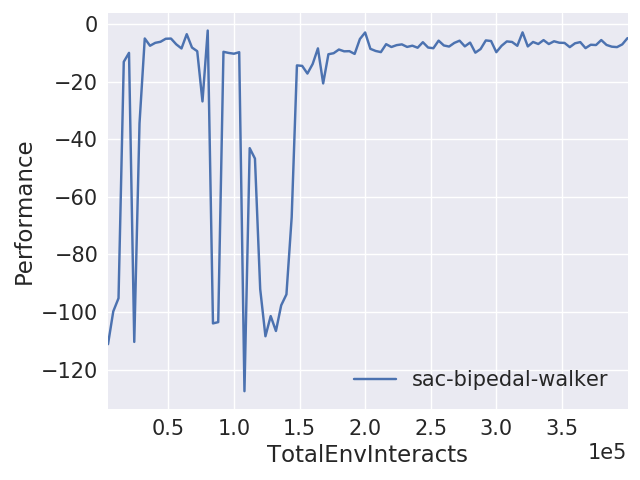
\includegraphics[width=\textwidth]{figures/rl-framework/sac-bipedal-walker.png}
         \caption{Spinning Up implementation (Default parameters) - Goal not achieved in 400.000 steps}
     \end{subfigure}
     \hfill
     \begin{subfigure}[c]{0.49\textwidth}
         \centering
         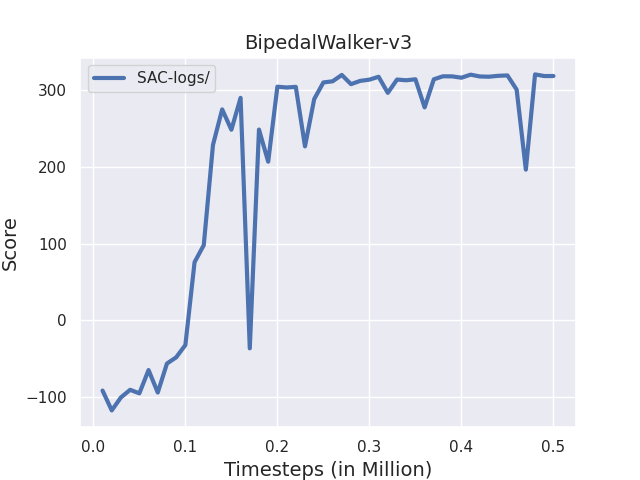
\includegraphics[width=\textwidth]{figures/rl-framework/sb3-sac-BipedalWalker-v3.png}
         \caption{Stable Baselines3 implementation (Tuned parameters) - Goal Achieved in 200.000 steps}
     \end{subfigure}
        \caption{Training Performance of Spinning Up vs Stable Baselines3 implementations of SAC. Goal Score: 300}
        \label{fig:spinup-vs-sb3}
\end{figure}

Moreover, the RL Baselines Zoo has the missing features of Spinning Up's training framework, namely hyperparameter optimization and continuing training of previously trained models. Therefore, SB3 will be the choice of RL Framework for this project from now on.

\section{State Estimator}

\section{Future Plans}

\subsection{Gym Environment}

In order to

\subsection{GoalEnv Interface}

\subsection{RL Algorithm Comparisons}



%%%%%%%%%%%%%%%%%%%%%%%%%%%%%%%%%%%%
%\chapter{Contribution}


%%%%%%%%%%%%%%%%%%%%%%%%%%%%%%%%%%%%
%\chapter{Experimental Results}


%%%%%%%%%%%%%%%%%%%%%%%%%%%%%%%%%%%%
%\chapter{Conclusion}



%% bibliography
\bibliographystyle{unsrt}
\setlength\bibsep{3pt}
\bibliography{bibliography}


%% appendix
\appendix
\addtocontents{toc}{\protect\setcounter{tocdepth}{0}}
\chapter{Sail Trim Approach}
In this chapter, a proposed extension to the broader "Automation and Intelligent Optimisation in High Performance Sailing Boats" project will be described. This Sail Trim Approach was my proposed master's thesis topic, but together with my supervisors, we decided to continue the Reinforcement Learning Approach instead.

\section{Introduction}
Sail trim is the biggest factor in the speed of the boat. An autopilot with a good sail trim would go faster than an expert human skipper with a bad sail trim. With a camera at the back of the boat looking at the main sail, we can train a model that can predict whether the main sail trim is good, too loose, or too tight.

Judging the sail trim is easy to a trained eye, but depending on the wind conditions, might require a lot of attention if the wind is gusty, or there is land or any obstacles nearby that might disturb the wind flow.
 
Full crews have dedicated people for sail trim, however it is hard to achieve constant good trim with shorthanded sailing with one or two people. This project would help shorthanded sailors, for cruising or racing, plus it can also be used for teaching sail trim to beginners.


\section{Literature Review}
In this section, a current overview of the relevant topics related to the proposed Sail Trim Approach (\ref{LR:TL}, \ref{LR:IG}, and \ref{LR:AST}) are presented. Transfer Learning is a suggested technique to be used in Sail Trim Approach so that the model can be trained with less collected data. Integrated Gradients is an Explainable AI technique which can be used for understanding what the sail trim model is learning to check if its correct. Lastly, Assisted Sail Trim is a system used in cruising yachts that is somewhat similar to the proposed Sail Trim Approach.

\subsection{Transfer Learning} \label{LR:TL}
Transfer learning is a method where a machine learning model trained for a task is used as a starting point for another task.\cite{brownlee_2019} In our context, instead of training a model from ground up, transfer learning can be utilized by building up on a model that was previously trained for a large scale image classification task. The idea behind transfer learning for imaging is that if a model is trained on a large and general enough dataset, it can serve as a generic model of the visual world. \cite{TF:TL} This generic model can be trained much more easily to classify different sail trims thanks to its advantages. 

Lisa Torrey and Jude Shavlik explain in their book the 3 advantages of transfer learning and how it improves model learning \cite{10.5555/1803899}, which can be seen in Figure \ref{fig:TL}.

\begin{figure}[h]
\centering
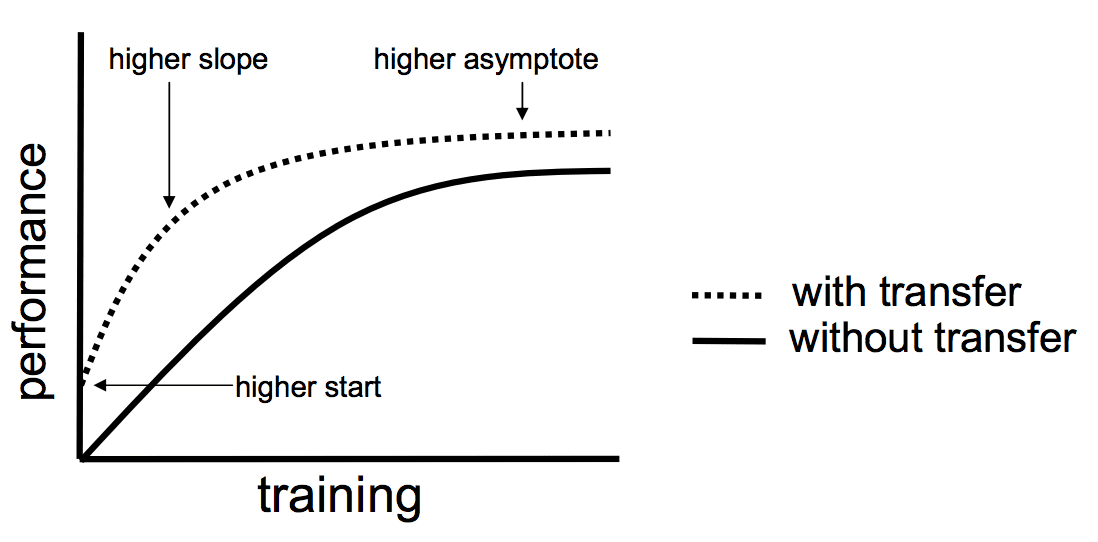
\includegraphics[width = 0.7\hsize]{figures/transfer-learning.png}
\caption{Transfer learning performance improvements \cite{10.5555/1803899}}
\label{fig:TL}
\end{figure}

\begin{enumerate}
  \item \textbf{Higher start:} The initial performance is better 
  \item \textbf{Higher slope:} The model improves faster 
  \item \textbf{Higher asymptote:} The converged performance is better 
\end{enumerate}

\begin{figure}[h]
\centering
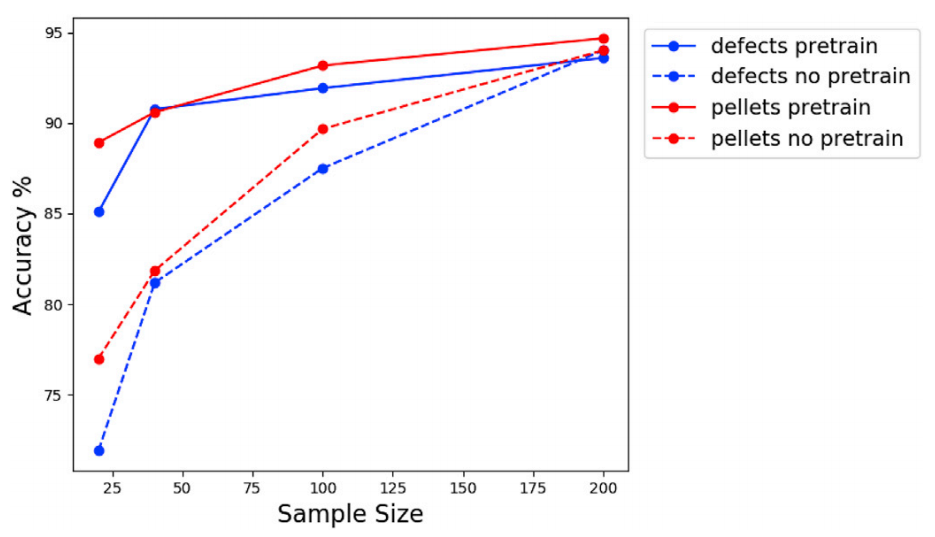
\includegraphics[width = 0.7\hsize]{figures/transfer learning results.png}
\caption{Affect of transfer learning on accuracy vs sample size \cite{ZHU2021104269}}
\label{fig:TL-results}
\end{figure}

Theoretically, using transfer learning the deep learning models converge much faster, as seen in Figure \ref{fig:TL}. This means that models can be trained with a lot less data. In their study, Wenbo et al. examines the transfer learning for image classification's impact on training sample size. \cite{ZHU2021104269} Wenbo et al. conclude that the deep learning models can achieve over 90\% accuracy for image classification tasks by using less than 100 samples utilizing transfer learning, significantly lower than the previous rule of thumb of 1000 samples per class. Wenbo et al.'s results graph of accuracy vs sample size, with and without transfer learning can be seen in Figure \ref{fig:TL-results}.

\subsection{Integrated Gradients} \label{LR:IG}
Integrated Gradients is an explainable AI technique to help understand what the model is learning, which can be used in any differentiable model such as images, text or structured data. \cite{TF:IG} The suggested usage in the sail trim approach is on images, to see whether the model is learning the expected features. The technique is easy to implement, and requires no modifications on the original network, only requires some calls to the standard gradient operator. \cite{IGpaper} An example of Integrated gradients used on images can be seen in Figure \ref{fig:IG}. 

\begin{figure}[h]
\centering
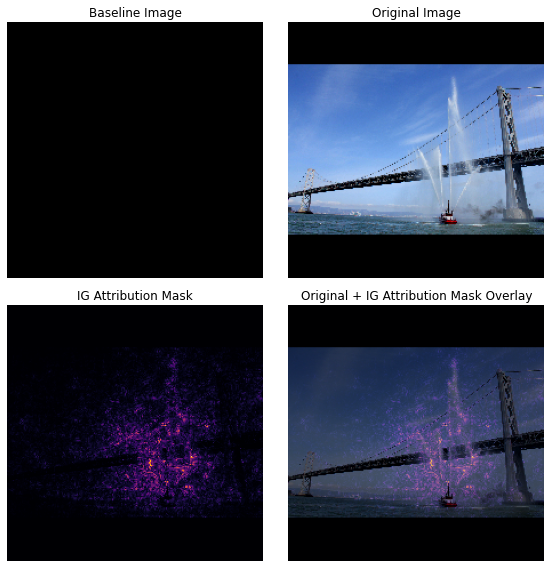
\includegraphics[width = 0.7\hsize]{figures/IG_fireboat.png}
\caption{Integrated Gradients example \cite{TF:IG}}
\label{fig:IG}
\end{figure}

When the models do not perform as expected, or just to see what the models have learned, Integrated Gradients is a nice technique to have to be able to understand and debug the models: either by regularization or gathering more and better balanced data.

\subsection{Jeanneau \& Harken Assisted Sail Trim} \label{LR:AST}
A somewhat similar idea to the sail trim approach has been done as a collaboration with Jeanneau and Harken in 2015, \cite{harkenAST} which won the Pittman Innovation Award. \cite{pittman_awards}
The Assisted Sail Trim (AST) system has several components. The relevant component to this project focuses on maintaining the rough trim of the sails by adjusting the sheets depending on the apparent wind measured by on-board electronics. An illustration of this can be seen in Figure~\ref{fig:AST}.

\begin{figure}[h]
\centering
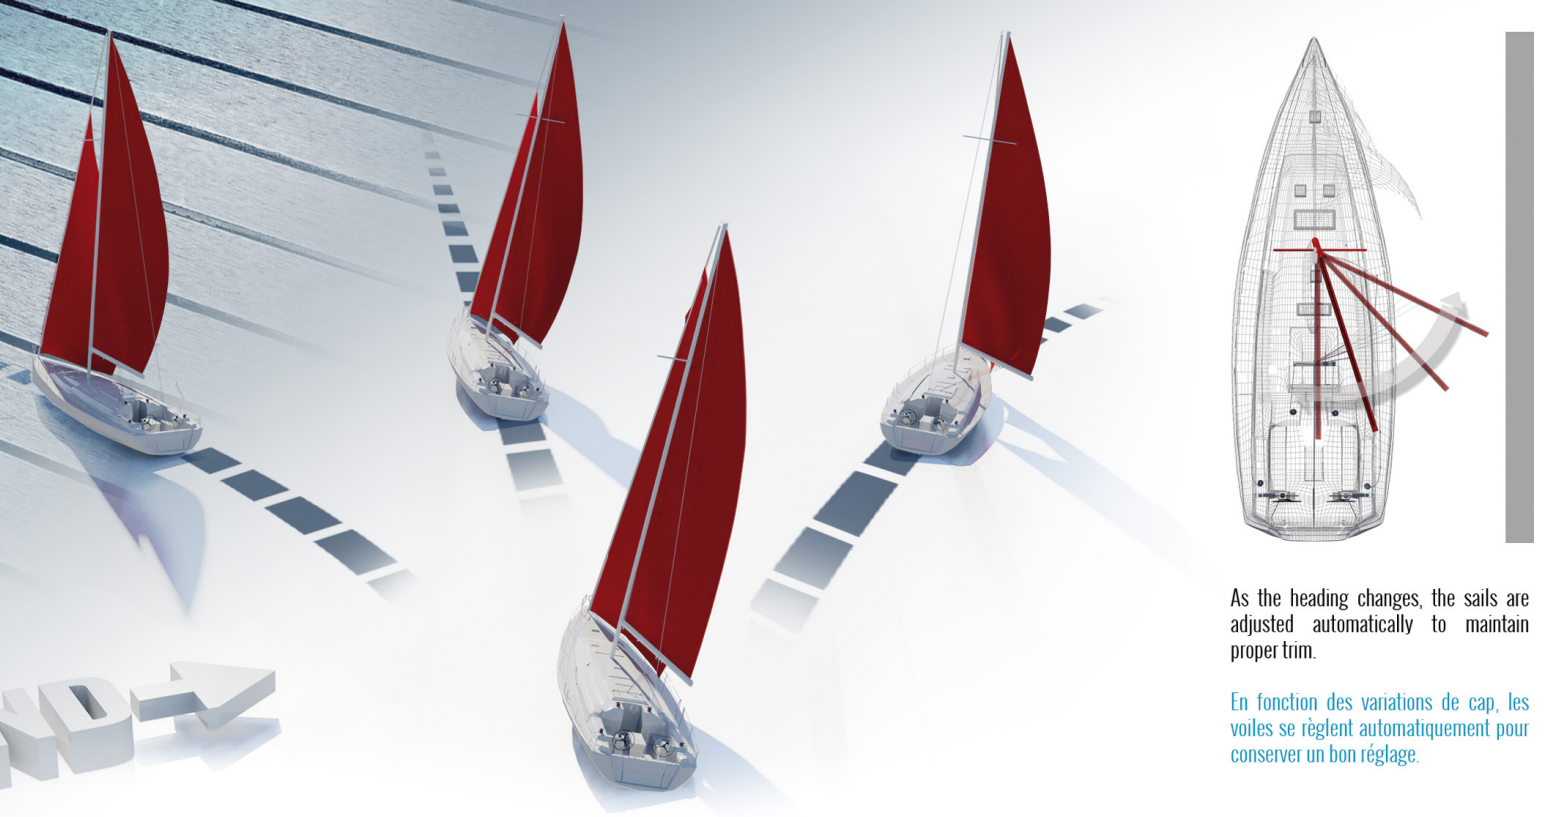
\includegraphics[width = \hsize]{figures/AST.png}
\caption{Assisted Sail Trim - apparent wind sail adjustment \cite{ASTbrochure}}
\label{fig:AST}
\end{figure}

AST is only available on the 2015 Jeanneau Sun Odyssey 519, and it is discontinued. It also did not utilize machine learning, required much more electronics and budget than a single camera, and it was specific to the sailboat, not transferable. In addition, the sails can have vastly different shapes even in similar sheet positions, resulting in great performance difference. The proposed sail trim approach focuses on the fine sail trim, rather than the coarse trim achieved in AST.

Another difference between AST and the suggested sail trim approach is that AST system can communicate with the winches, and automatically adjust the main sheet. Suggested sail trim approach will not communicate with the rest of the onboard electronics, and rely on the crew to take actions. Although this is less user friendly, it has its own advantages. Two use cases of the sail trim approach are education and competition. Making the crew do the trim by giving trim suggestion will be more educational than doing it for them. Plus automated sail trim is not allowed in some class rules, so this project can be used in competitions among wider sailboat classes.

\section{Sail Trim Background}
As explained in section \ref{LR:AST}, the sails can have vastly different shapes in similar boom and sheet positions as can be seen in Figure~\ref{fig:mainsail-trim}. There are a lot of reasons why a sail trim might be off. For example the sail might not be cut properly, or the mast position and mast bend might not be optimal for the weather conditions. But these are pretty unlikely, and most likely, it is the mainsail controls that can be adjusted on the go that cause bad trim. Below are some notable reasons of bad mainsail trim on the go.

\begin{figure}[h]
\centering
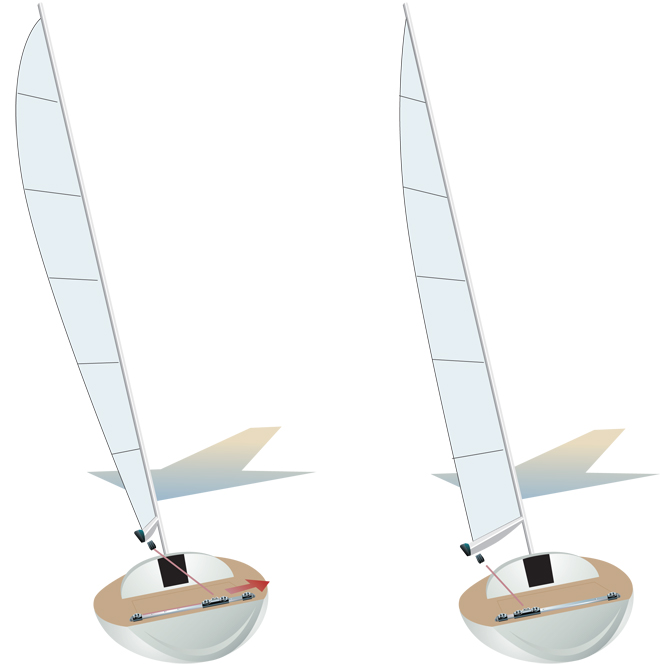
\includegraphics[width = 0.6\hsize]{figures/sail-trim-approach/mainsail-trim-back.jpg}
\caption{Good(left) and bad(right) light wind mainsail trim \cite{img:mainsail-trim-back}}
\label{fig:mainsail-trim}
\end{figure}

\noindent Main sail might be too strained because of:
\begin{itemize}
  \item The main sheet is pulled in too much
  \item Boom vang is too tight
  \item Main sail traveller is not utilized correctly
\end{itemize}

\noindent Main sail might be too loose because of:
\begin{itemize}
  \item The main sheet is not pulled enough
  \item Boom vang is too loose
  \item Main sail is not fully up to the top of the mast
\end{itemize}

There are other mainsail controls that affect the trim such as cunningham and outhaul, but those depend a lot on the boat class, and even in same boat class, different sailmakers have different suggestions on how to utilize them. The mentioned mainsail controls can be seen in Figure \ref{fig:mainsail-controls}.

\begin{figure}[h]
\centering
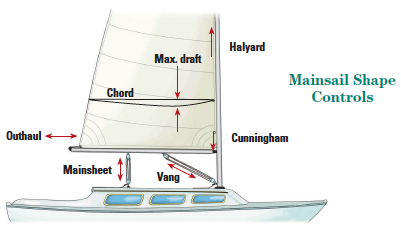
\includegraphics[width = 0.7\hsize]{figures/sail-trim-approach/mainsail-shape-controls.png}
\caption{Mainsail controls that affect trim \cite{img:mainsail-shape-controls}}
\label{fig:mainsail-controls}
\end{figure}

\section{Sail Trim Capture System}

The suggested camera placement is at the center back of the boat, possibly at the bimini top, as shows in Figure \ref{fig:camera-pos}. A camera from this angle will see a similar view of the sails with Figure \ref{fig:telltales}.

\begin{figure}[h]
\centering
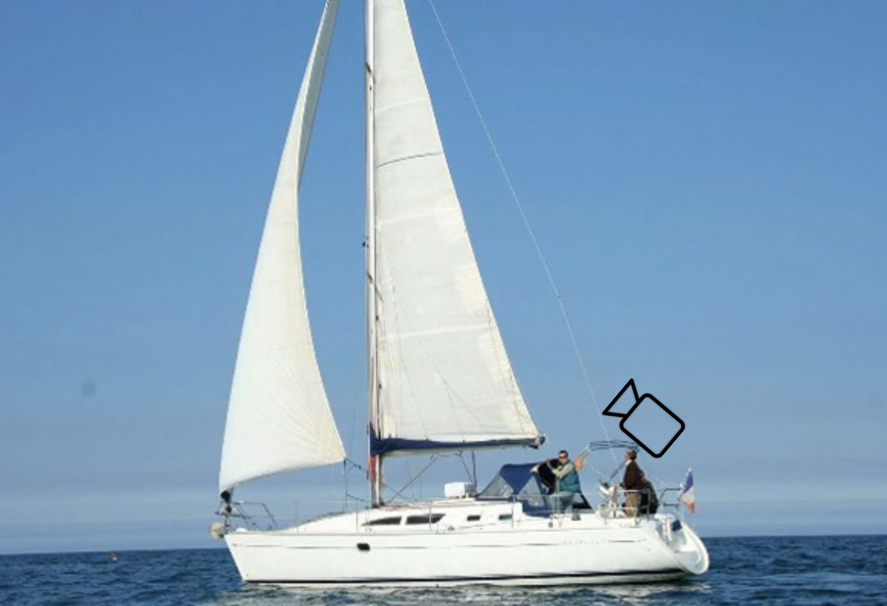
\includegraphics[width = 0.7\hsize]{figures/sail-trim-approach/camera-position.png}
\caption{Camera position}
\label{fig:camera-pos}
\end{figure}

\begin{figure}[h]
\centering
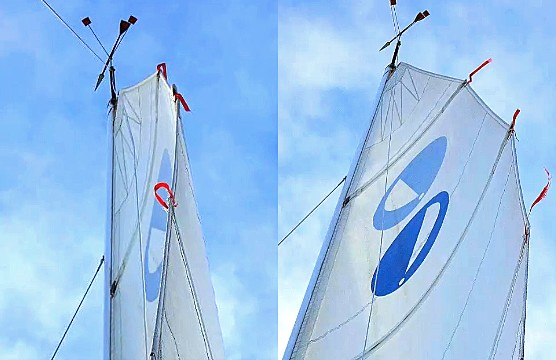
\includegraphics[width = 0.8\hsize]{figures/sail-trim-approach/telltales.jpg}
\caption{Camera's view of a bad(left) and good(right) light wind mainsail trim \cite{img:telltales}}
\label{fig:telltales}
\end{figure}

The easiest way to tell if the trim is good for a human is to look at the red telltales at the back of the sails, see Figure \ref{fig:telltales}. The most important one is the topmost one. If the telltales are flying straight back, it means that the air is coming out of the sails alright. However if the telltale is going to the back of the sails, it shows us that the wind flow at the back of the sails are not optimal, meaning the trim is sub-optimal and the sails need to be loosened.

For a machine, the easiest way to check trim might be comparing the areas of sail and the sky. In Figure \ref{fig:telltales}, you'll notice that Assuming a clear sky, by only comparing the number of blue pixels(sky) and the number of whiter pixels(sails), a very simple model can tell the difference between a good and a bad trim.

Using the state of the art image classification models, we can achieve much better results, theoretically learning the sail trim for different wind and weather conditions, apparent wind angles, maybe even across different boats.


\section{Suggested Timeline}

The suggested timeline and some additional details for this project, planned considering the available time for Imperial MSc thesis projects can be seen in Figures \ref{fig:sta-plan1} and \ref{fig:sta-plan2}.

\begin{figure}[h]
\centering
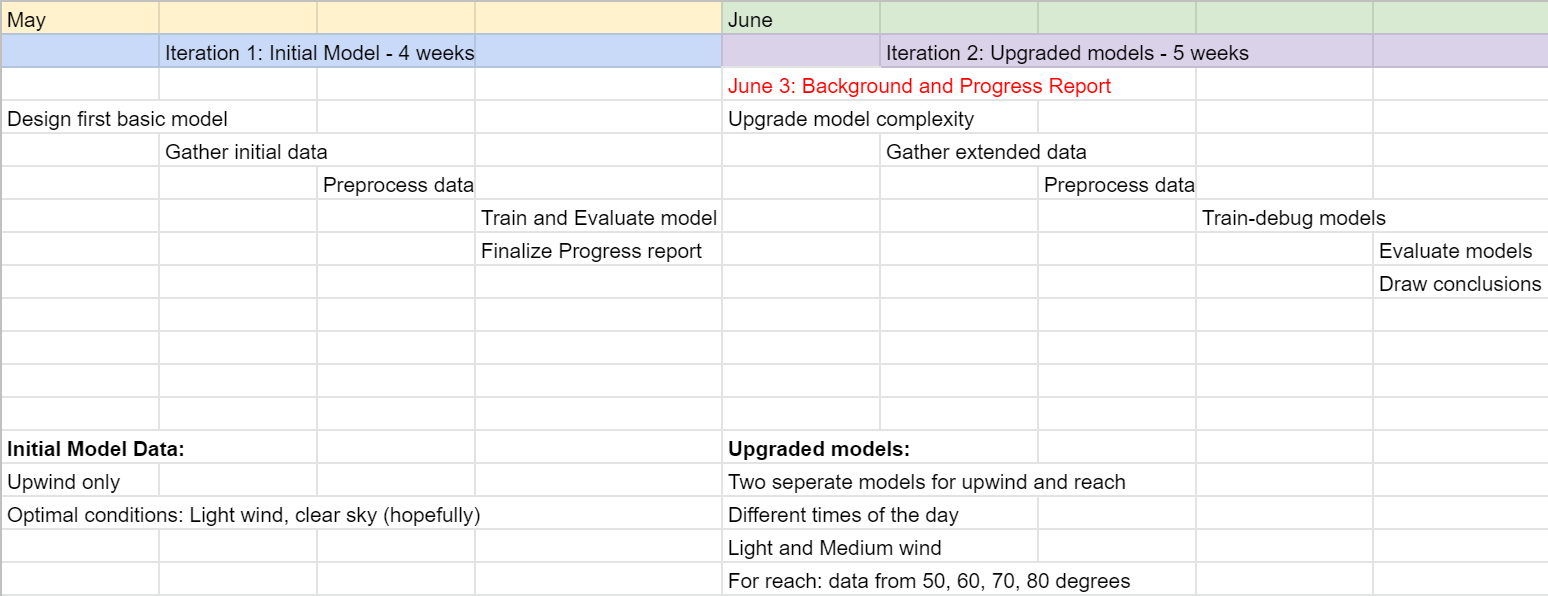
\includegraphics[width = \hsize]{figures/sail-trim-approach/plan1.png}
\caption{Suggested plan - Iterations 1 and 2}
\label{fig:sta-plan1}
\end{figure}

Iteration 1 aims to build a simple Proof of Concept that machine learning models can classify good and bad sail trims. After the initial Proof of Concept, the models are extended in Iteration 2. If the expected results are not met in the first iteration, using Integrated Gradients explained in section \ref{LR:IG}, one can see what the models have learned, assess if the learnt features are correct, and balance the dataset with more data countering the false features.

\begin{figure}[h]
\centering
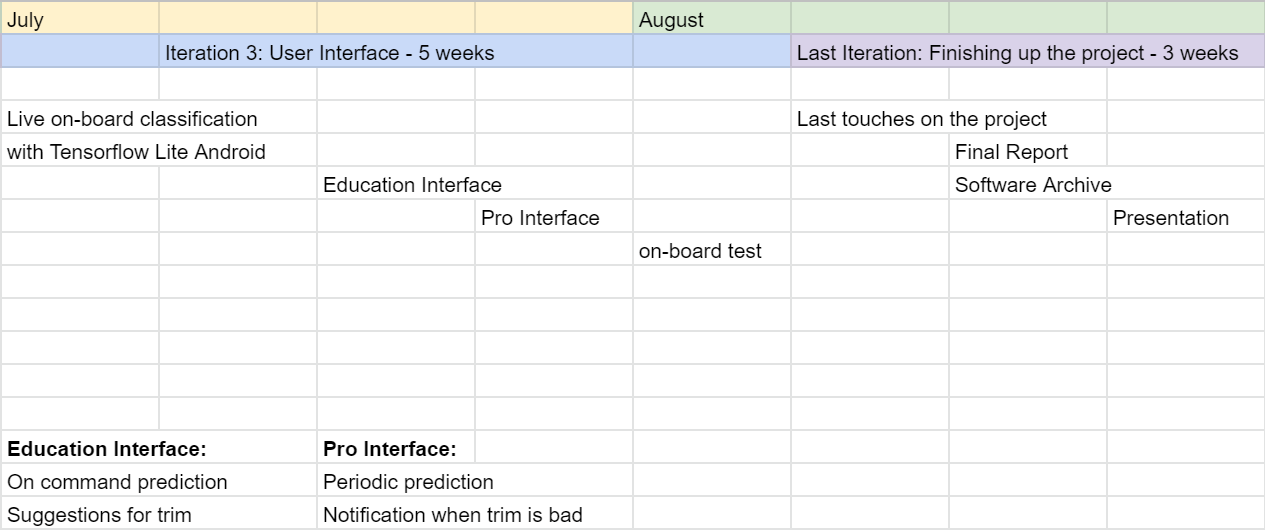
\includegraphics[width = \hsize]{figures/sail-trim-approach/plan2.png}
\caption{Suggested plan - Iterations 3 and 4}
\label{fig:sta-plan2}
\end{figure}

Iteration 3 aims to implement the models live on-board using a smartphone, including two different interfaces for education and professional use cases. Iteration 4 contains a buffer week if anything goes wrong for the project, then some time for project submission preparations, namely the code submission to software archive, final report, and the final presentation.

For more information about the Sail Trim Approach, you can email me at:\\
\href{mailto:doruktaneli97@gmail.com}{doruktaneli97@gmail.com}

\end{document}
